% Judul dokumen
\title{Buku Tugas Akhir ITS}
\author{Aptanagi, Urdhanaka}

% Pengaturan ukuran teks dan bentuk halaman dua sisi
\documentclass[12pt,twoside]{report}
\setcounter{secnumdepth}{3}
\setcounter{tocdepth}{2}

% Pengaturan ukuran halaman dan margin
\usepackage[a4paper,top=30mm,left=30mm,right=20mm,bottom=25mm]{geometry}

% Pengaturan ukuran spasi
\usepackage[singlespacing]{setspace}

% Pengaturan detail pada file PDF
\usepackage[pdfauthor={\@author},bookmarksnumbered,pdfborder={0 0 0}]{hyperref}

% Pengaturan jenis karakter
\usepackage[T1]{fontenc}
\usepackage[utf8]{inputenc}

% Pengaturan pewarnaan
\usepackage[table,xcdraw]{xcolor}

% Pengaturan kutipan artikel
\usepackage[style=apa, backend=biber]{biblatex}

\usepackage[titles]{tocloft}
\setlength{\cftsecindent}{1em}
\setlength{\cftsubsecindent}{2em}
\setlength{\cftsubsubsecindent}{3em}
\setlength{\cftbeforechapskip}{1.5ex}
\setlength{\cftbeforesecskip}{1ex}
\setlength{\cftbeforesubsecskip}{1ex}
\setlength{\cftbeforesubsubsecskip}{1ex}
\setlength{\cftbeforetoctitleskip}{0cm}
\setlength{\cftbeforeloftitleskip}{4ex}
\setlength{\cftafterloftitleskip}{0cm}
\setlength{\cftbeforelottitleskip}{0cm}
\setlength{\cftfigindent}{0pt}
\setlength{\cfttabindent}{0pt}
\renewcommand{\cfttoctitlefont}{\hfill\Large\bfseries}
\renewcommand{\cftaftertoctitle}{\hfill}
\renewcommand{\cftloftitlefont}{\hfill\Large\bfseries}
\renewcommand{\cftafterloftitle}{\hfill}
\renewcommand{\cftlottitlefont}{\hfill\Large\bfseries}
\renewcommand{\cftafterlottitle}{\hfill}
\renewcommand{\cftchappresnum}{BAB\ }
\setlength{\cftchapnumwidth}{3.2em}

% Package lainnya
\usepackage{changepage}
\usepackage{enumitem}
\usepackage{eso-pic}
\usepackage{txfonts} % Font times
\usepackage{etoolbox}
\usepackage{graphicx}
\usepackage{lipsum}
\usepackage{longtable}
\usepackage{tabularx}
\usepackage{wrapfig}
\usepackage{float}

% Definisi untuk "Hati ini sengaja dikosongkan"
\patchcmd{\cleardoublepage}{\hbox{}}{
  \thispagestyle{empty}
  \vspace*{\fill}
  \begin{center}\textit{[Halaman ini sengaja dikosongkan]}\end{center}
  \vfill}{}{}

% Pengaturan penomoran halaman
\usepackage{fancyhdr}
\fancyhf{}
\renewcommand{\headrulewidth}{0pt}
\pagestyle{fancy}
\fancyfoot[LE,RO]{\thepage}
\patchcmd{\chapter}{plain}{fancy}{}{}
\patchcmd{\chapter}{empty}{plain}{}{}

% Command untuk bulan
\newcommand{\MONTH}{%
  \ifcase\the\month
  \or Januari% 1
  \or Februari% 2
  \or Maret% 3
  \or April% 4
  \or Mei% 5
  \or Juni% 6
  \or Juli% 7
  \or Agustus% 8
  \or September% 9
  \or Oktober% 10
  \or November% 11
  \or Desember% 12
  \fi}
\newcommand{\ENGMONTH}{%
  \ifcase\the\month
  \or January% 1
  \or February% 2
  \or March% 3
  \or April% 4
  \or May% 5
  \or June% 6
  \or July% 7
  \or August% 8
  \or September% 9
  \or October% 10
  \or November% 11
  \or December% 12
  \fi}

% Pengaturan format judul bab
\usepackage{titlesec}
\titleformat{\chapter}[block]{\bfseries\Large}{BAB \centering\arabic{chapter}}{1ex}{\vspace{0ex}\centering}
\titleformat{\section}{\bfseries\large}{\MakeUppercase{\thesection}}{1ex}{\vspace{1ex}}
\titleformat{\subsection}{\bfseries\large}{\MakeUppercase{\thesubsection}}{1ex}{}
\titleformat{\subsubsection}{\bfseries\large}{\MakeUppercase{\thesubsubsection}}{1ex}{}
\titleformat{\subsubsubsection}{\bfseries\large}{\MakeUppercase{\thesubsubsubsection}}{1ex}{}
\titlespacing{\chapter}{0ex}{-5ex}{4ex}
\titlespacing{\section}{0ex}{1ex}{0ex}
\titlespacing{\subsection}{0ex}{0.5ex}{0ex}
\titlespacing{\subsubsection}{0ex}{0.5ex}{0ex}
\titlespacing{\subsubsubsection}{0ex}{0.5ex}{0ex}

\counterwithin{figure}{chapter}
\counterwithin{table}{chapter}

\usepackage{listings}
\definecolor{comment}{RGB}{0,128,0}
\definecolor{string}{RGB}{255,0,0}
\definecolor{keyword}{RGB}{0,0,255}
\renewcommand{\lstlistingname}{Kode Sumber}
\lstdefinestyle{codestyle}{
  commentstyle=\color{comment},
  stringstyle=\color{string},
  keywordstyle=\color{keyword},
  basicstyle=\footnotesize\ttfamily,
  numbers=left,
  numberstyle=\tiny,
  numbersep=5pt,
  frame=lines,
  breaklines=true,
  prebreak=\raisebox{0ex}[0ex][0ex]{\ensuremath{\hookleftarrow}},
  showstringspaces=false,
  upquote=true,
  tabsize=2,
  captionpos=b,
  % xleftmargin=5mm,
}
\lstdefinestyle{clistyle}{
  basicstyle=\footnotesize\ttfamily,
  numbers=none,
  frame=single,
  breaklines=true,
  prebreak=\raisebox{0ex}[0ex][0ex]{\ensuremath{\hookleftarrow}},
  captionpos=b,
}
\lstset{
  aboveskip=15pt,
  style=codestyle
}

% lstlistoflistings configuration
\makeatletter
\renewcommand{\l@lstlisting}[2]{
  \@dottedtocline{1}{0em}{2.3em}{#1}{#2}%
}
\makeatother

% Atur variabel berikut sesuai namanya

% nama
\newcommand{\name}{Urdhanaka Aptanagi}
\newcommand{\authorname}{Aptanagi, Urdhanaka}
\newcommand{\nickname}{Elon}
\newcommand{\advisor}{Royyana Muslim Ijtihadie, S.Kom., M.Kom., Ph.D.}
\newcommand{\coadvisor}{Ary Mazharuddin Shiddiqi, S.Kom., M.Comp.Sc., Ph.D.}
\newcommand{\examinerone}{Dr. Galileo Galilei, S.T., M.Sc}
\newcommand{\examinertwo}{Friedrich Nietzsche, S.T., M.Sc}
\newcommand{\examinerthree}{Alan Turing, ST., MT}
\newcommand{\headofdepartment}{Ary Mazharuddin Shiddiqi, S.Kom., M.Comp.Sc., Ph.D.}

  % Dosen Pembimbing&:& 1. Royyana Muslim Ijtihadie, S.Kom., M.Kom., Ph.D.\\

% identitas
\newcommand{\nrp}{5025211123}
\newcommand{\advisornip}{19770824 200304 1 001}
\newcommand{\coadvisornip}{19810620 200501 1 003}
\newcommand{\examineronenip}{18560710 194301 1 001}
\newcommand{\examinertwonip}{18560710 194301 1 001}
\newcommand{\examinerthreenip}{18560710 194301 1 001}
\newcommand{\headofdepartmentnip}{19810620 200501 1 003}

% judul
\newcommand{\tatitle}{IMPLEMENTASI \emph{MULTI-TENANCY} UNTUK PROVISIONING KLASTER KUBERNETES}
\newcommand{\engtatitle}{\emph{MULTI-TENANCY IMPLEMENTATION FOR KUBERNETES CLUSTER PROVISIONING}}

% tempat
\newcommand{\place}{Surabaya}

% jurusan
\newcommand{\studyprogram}{Teknik Informatika}
\newcommand{\engstudyprogram}{Informatics}

% fakultas
\newcommand{\faculty}{Fakultas Teknologi Elektro dan Informatika Cerdas}
\newcommand{\engfaculty}{Faculty of Intelligent Electrical and Informatics Technology}

% singkatan fakultas
\newcommand{\facultyshort}{FTEIC}
\newcommand{\engfacultyshort}{ELECTICS}

% departemen
\newcommand{\department}{Teknik Informatika}
\newcommand{\engdepartment}{Informatics}

% kode mata kuliah
\newcommand{\coursecode}{EF234801}

% Tambahkan format tanda hubung yang benar di sini
\hyphenation{
  ro-ket
  me-ngem-bang-kan
  per-hi-tu-ngan
  tek-no-lo-gi
  me-la-ku-kan
  ber-so-si-al-i-sa-si
  peng-hu-bung
  pro-ses
  No-pem-ber
  ber-na-ma
  di-kem-bang-kan
  klas-ter
  ge-ne-rik
  kon-ku-ren-si
  ku-be-con-trol-ler-ma-na-ger
  be-ri-kut
  per-be-da-an
  se-per-ti
  me-mu-dah-kan
  le-bih
  peng-gu-na-an
  Peng-gu-na-an
  Ble-ki-nge
  di-te-rus-kan
}


% Menambahkan resource daftar pustaka
\addbibresource{pustaka/pustaka.bib}

% Isi keseluruhan dokumen
\begin{document}

% Sampul luar Bahasa Indonesia
\newcommand\covercontents{sampul/konten-id.tex}
\AddToShipoutPictureBG*{
  \AtPageLowerLeft{
    % Ubah nilai berikut jika posisi horizontal background tidak sesuai
    \hspace{-3.25mm}

    % Ubah nilai berikut jika posisi vertikal background tidak sesuai
    \raisebox{0mm}{
      
\includegraphics[width=\paperwidth,height=\paperheight]{sampul/gambar/sampul-luar.png}
    }
  }
}

% Menyembunyikan nomor halaman
\thispagestyle{empty}

% Pengaturan margin untuk menyesuaikan konten sampul
\newgeometry{
  top=55mm,
  left=30mm,
  right=20mm,
  bottom=20mm
}

\begin{flushleft}

  % Pemilihan font sans serif
  \sffamily

  % Pemilihan warna font putih
  \color{white}

  % Pemilihan font bold
  \fontseries{bx}
  \selectfont
  \begin{spacing}{1.5}
    \input{\covercontents}
  \end{spacing}

\end{flushleft}

\restoregeometry


% Atur ulang penomoran halaman
\setcounter{page}{1}

% Sampul dalam Bahasa Indonesia
\renewcommand\covercontents{sampul/konten-id-dalam.tex}
\AddToShipoutPictureBG*{
  \AtPageLowerLeft{
    % Ubah nilai berikut jika posisi horizontal background tidak sesuai
    \hspace{-4mm}

    % Ubah nilai berikut jika posisi vertikal background tidak sesuai
    \raisebox{0mm}{
      
\includegraphics[width=\paperwidth,height=\paperheight]{sampul/gambar/sampul-luar-tipis.png}
    }
  }
}

% Menyembunyikan nomor halaman
\thispagestyle{empty}

% Pengaturan margin untuk menyesuaikan konten sampul
\newgeometry{
  top=65mm,
  left=30mm,
  right=30mm,
  bottom=20mm
}

\begin{flushleft}

  % Pemilihan font sans serif
  \sffamily

  % Pemilihan font bold
  \fontseries{bx}
  \selectfont
  \begin{spacing}{1.5}
    \input{\covercontents}
  \end{spacing}

\end{flushleft}

\restoregeometry

\cleardoublepage

% Sampul dalam Bahasa Inggris
\renewcommand\covercontents{sampul/konten-en.tex}
\AddToShipoutPictureBG*{
  \AtPageLowerLeft{
    % Ubah nilai berikut jika posisi horizontal background tidak sesuai
    \hspace{-4mm}

    % Ubah nilai berikut jika posisi vertikal background tidak sesuai
    \raisebox{0mm}{
      
\includegraphics[width=\paperwidth,height=\paperheight]{sampul/gambar/sampul-luar-tipis.png}
    }
  }
}

% Menyembunyikan nomor halaman
\thispagestyle{empty}

% Pengaturan margin untuk menyesuaikan konten sampul
\newgeometry{
  top=65mm,
  left=30mm,
  right=30mm,
  bottom=20mm
}

\begin{flushleft}

  % Pemilihan font sans serif
  \sffamily

  % Pemilihan font bold
  \fontseries{bx}
  \selectfont
  \begin{spacing}{1.5}
    \input{\covercontents}
  \end{spacing}

\end{flushleft}

\restoregeometry

\cleardoublepage

% Label tabel dan gambar dalam bahasa indonesia
\renewcommand{\figurename}{Gambar}
\renewcommand{\tablename}{Tabel}

% Pengaturan ukuran indentasi paragraf
\setlength{\parindent}{2em}

% Pengaturan ukuran spasi paragraf
\setlength{\parskip}{1ex}

% Nomor halaman pembuka dimulai dari sini
\pagenumbering{roman}

% Lembar pengesahan dan pernyataan-keaslian
\begin{center}
  \large
  \textbf{LEMBAR PENGESAHAN}
\end{center}

% Menyembunyikan nomor halaman
\thispagestyle{empty}

\begin{center}
  \textbf{\tatitle{}}
\end{center}

\begingroup
% Pemilihan font ukuran small
\small

\begin{center}
  \textbf{TUGAS AKHIR}
  \\Diajukan untuk memenuhi salah satu syarat \\
  memperoleh gelar Sarjana Teknik pada \\
  Program Studi S-1 \studyprogram{} \\
  Departemen \department{} \\
  Fakultas \faculty{} \\
  Institut Teknologi Sepuluh Nopember
\end{center}

\begin{center}
  Oleh: \textbf{\name{}}
  \\NRP. \nrp{}
\end{center}

\begin{center}
  Disetujui oleh Tim Penguji Tugas Akhir:
\end{center}

\begingroup
% Menghilangkan padding
\setlength{\tabcolsep}{0pt}

\noindent
\begin{tabularx}{\textwidth}{X l}
  \advisor{}               & (Pembimbing I)                      \\
  NIP: \advisornip{}       &                                     \\
                           & ................................... \\
                           &                                     \\
                           &                                     \\
  \coadvisor{}             & (Pembimbing II)                     \\
  NIP: \coadvisornip{}     &                                     \\
                           & ................................... \\
                           &                                     \\
                           &                                     \\
  \examinerone{}.          & (Penguji I)                         \\
  NIP: \examineronenip{}   &                                     \\
                           & ................................... \\
                           &                                     \\
                           &                                     \\
  \examinertwo{}.          & (Penguji II)                        \\
  NIP: \examinertwonip{}   &                                     \\
                           & ................................... \\
                           &                                     \\
                           &                                     \\
  \examinerthree{}.        & (Penguji III)                       \\
  NIP: \examinerthreenip{} &                                     \\
                           & ................................... \\
\end{tabularx}
\endgroup

\begin{center}
  Mengetahui, \\
  Kepala Departemen \department{} \facultyshort{} - ITS\\

  \vspace{8ex}

  \underline{\headofdepartment{}.} \\
  NIP. \headofdepartmentnip{}
\end{center}

\begin{center}
  \textbf{\MakeUppercase{\place{}}\\\MONTH{}, \the\year{}}
\end{center}
\endgroup

\cleardoublepage
\chapter*{PERNYATAAN ORISINALITAS}

\addcontentsline{toc}{chapter}{PERNYATAAN ORISINALITAS}

\vspace{2ex}

% Ubah paragraf-paragraf berikut sesuai dengan yang ingin diisi pada pernyataan keaslian

\noindent Yang bertanda tangan dibawah ini:

\noindent\begin{tabularx}{\textwidth}{l l X}
                         &   &                            \\
  Nama Mahasiswa / NRP   & : & \name{} / \nrp{}           \\
  Departemen             & : & \department{}              \\
  Dosen Pembimbing / NIP & : & \advisor{} / \advisornip{} \\
                         &   &                            \\
\end{tabularx}

Dengan ini menyatakan bahwa Tugas Akhir dengan judul "\tatitle{}" adalah hasil karya sendiri, berfsifat orisinal, dan ditulis dengan mengikuti kaidah penulisan ilmiah.

Bilamana di kemudian hari ditemukan ketidaksesuaian dengan pernyataan ini, maka saya bersedia menerima sanksi sesuai dengan ketentuan yang berlaku di Institut Teknologi Sepuluh Nopember.

\vspace{8ex}

\noindent\begin{tabularx}{\textwidth}{X l}
                     & \place{}, \MONTH{} \the\year{} \\
                     &                                   \\
  Mengetahui         &                                   \\
  Dosen Pembimbing   & Mahasiswa                         \\
                     &                                   \\
                     &                                   \\
                     &                                   \\
                     &                                   \\
                     &                                   \\
  \advisor{}         & \name{}                           \\
  NIP. \advisornip{} & NRP. \nrp{}                       \\
\end{tabularx}

\cleardoublepage

% Abstrak
\begin{center}
  \large\textbf{ABSTRAK}
\end{center}

\addcontentsline{toc}{chapter}{ABSTRAK}

\vspace{2ex}

\begingroup
% Menghilangkan padding
\setlength{\tabcolsep}{0pt}

\noindent
\begin{tabularx}{\textwidth}{l >{\centering}m{2em} X}
  Nama Mahasiswa    & : & \name{}         \\

  Judul Tugas Akhir & : & \tatitle{}      \\

  Pembimbing        & : & 1. \advisor{}   \\
                    &   & 2. \coadvisor{} \\
\end{tabularx}
\endgroup

% Ubah paragraf berikut dengan abstrak dari tugas akhir
Pada penelitian ini kami mengajukan \lipsum[1]

% Ubah kata-kata berikut dengan kata kunci dari tugas akhir
Kata Kunci: Roket, \emph{Anti-gravitasi}, Energi, Angkasa.

\cleardoublepage
\chapter*{ABSTRACT}

\addcontentsline{toc}{chapter}{ABSTRACT}

\vspace{2ex}

\begin{center}
  \large\textbf{\engtatitle{}}
\end{center}

\vspace{2ex}

\begingroup
% Menghilangkan padding
\setlength{\tabcolsep}{0pt}

\noindent
\begin{tabularx}{\textwidth}{l >{\centering}m{3em} X}
  \textbf{Name / NRP} & : & \textbf{\name{} / \nrp{}} \\
  \textbf{Department} & : & \textbf{\engdepartment{}} \\
  \textbf{Advisor I}  & : & \textbf{\advisor{}}       \\
  \textbf{Advisor II} & : & \textbf{\coadvisor{}}     \\
\end{tabularx}
\endgroup

\noindent
\textbf{Abstract}

% Ubah paragraf berikut dengan abstrak dari tugas akhir dalam Bahasa Inggris
Computing resources such as computers are not always in use or in idle
position. This can lead to computing resources waste. To prevent that,
a mechanism is needed to utilize these resources  by renting out the
idle resources to users in need. One of the tools that can be used is Kubernetes.
However, using Kubernetes usually requires fix amount of resources. In this study,
we propose a Kubernetes provisioning system in the form of virtual cluster. Virtual
cluster is an approach that allows computing resources to be provided on-demand. In
addition, multi-tenancy will also be implemented so that computing resources that are
rented can be used by more than one user. The result of this study is that the virtual
cluster provisioning system can be used as additional computing resources for its users
on-demand. In addition, user also shares computing resources with other users.

\vspace{2ex}
% Ubah kata-kata berikut dengan kata kunci dari tugas akhir dalam Bahasa Inggris
\noindent
\textbf{Keywords: Kubernetes, Multi-Tenancy, Virtual Cluster, Virtual Machine.}

\cleardoublepage

\chapter*{LEMBAR PENGESAHAN}

\addcontentsline{toc}{chapter}{KATA PENGANTAR}

\vspace{2ex}

% Ubah paragraf-paragraf berikut dengan isi dari kata pengantar

Puji dan syukur penulis panjatkan kepada Tuhan Yang Maha Esa karena atas rahmat
dan karunia-Nya, penulis dapat menyelesaikan laporan tugas akhir yang berjudul
"IMPLEMENTASI \emph{MULTI-TENANCY} UNTUK PROVISIONING KLASTER KUBERNETES" dengan
baik. Tugas akhir ini disusun sebagai persyaratan untuk memperoleh gelar sarjana
pada program studi Teknik Informatika Fakultas Teknologi Elektro dan Informatika
Cerdas Institut Teknologi Sepuluh Nopember. Penulisan tugas akhir ini tidak lepas
dari dukungan dan bantuan dari berbagai pihak.
Oleh karena itu, penulis mengucapkan terima kasih kepada:

\begin{enumerate}[nolistsep]

  \item Bapak Royyana Muslim Ijtihadie, S.Kom., M.Kom., Ph.D. selaku dosen pembimbing
    utama penulis dan Bapak Ary Mazharuddin Shiddiqi, S.Kom., M.Comp.Sc., Ph.D. selaku dosen
    pembimbing kedua penulis yang telah membantu penulis dalam menyelesaikan Tugas Akhir.

  \item Keluarga penulis, Ibu penulis, Bapak penulis dan dua Saudara penulis yang telah 
    memberikan dukungan kepada penulis. \lipsum[3][1-2]

  \item Teman-teman "\emph{Backstreet Boys}"
    
  \item Alwan Raihan, Bhatara Arundaya, Orisvio Revanda, S.T., Rayhan Rizky, dan Tigo Yoga
    selaku teman-teman "Ahmad Dahlan" yang telah memberikan semangat dan dukungan kepada
    penulis selama pengerjaan.

  \item Adam Daffa, Hanif Setyadi, Muhammad Rafi, Orisvio Revanda, S.T., dan Tio
    Widayat, S.H., selaku teman "Risin Inti Diing". Terima kasih penulis ucapkan
    sebesar-besarnya.

\end{enumerate}

Laporan tugas akhir ini jauh dari kata sempurna, oleh karena itu penulis
sangat terbuka terhadap kritik dan saran yang membangun. Akhir kata, semoga
laporan tugas akhir ini dapat memberikan dampak dan manfaat yang baik kepada
seluruh pihak yang memerlukan.

\begin{flushright}
  \begin{tabular}[b]{c}
    \place{}, \MONTH{} \the\year{} \\
    \\
    \\
    \\
    \\
    \name{}
  \end{tabular}
\end{flushright}

\cleardoublepage

% Daftar isi
\renewcommand*\contentsname{DAFTAR ISI}
\phantomsection
\addcontentsline{toc}{chapter}{\contentsname}
\tableofcontents
\cleardoublepage

% Daftar gambar
\renewcommand*\listfigurename{DAFTAR GAMBAR}
\phantomsection
\addcontentsline{toc}{chapter}{\listfigurename}
\renewcommand{\addvspace}[1]{}%
\listoffigures
\cleardoublepage

% Daftar tabel
\renewcommand*\listtablename{DAFTAR TABEL}
\phantomsection
\addcontentsline{toc}{chapter}{\listtablename}
\listoftables
\cleardoublepage

\renewcommand*\lstlistlistingname{DAFTAR KODE SUMBER DAN KODE PERINTAH}
\phantomsection
\addcontentsline{toc}{chapter}{\lstlistlistingname}
\lstlistoflistings
\cleardoublepage

% Nomor halaman isi dimulai dari sini
\pagenumbering{arabic}

% Bab 1 pendahuluan
\chapter{PENDAHULUAN}
\label{chap:pendahuluan}

% Ubah bagian-bagian berikut dengan isi dari pendahuluan

Penelitian ini dilatarbelakangi oleh \lipsum[1][1-5]

\section{Latar Belakang}
\label{sec:latarbelakang}

Pesatnya perkembangan roket yang merupakan \lipsum[1]

\lipsum[2]

\section{Permasalahan}
\label{sec:permasalahan}

Dari permasalahan tersebut maka \lipsum[1][1-6]

\section{Tujuan}
\label{sec:Tujuan}

Tujuan dari \lipsum[1][1-3] adalah:

\begin{enumerate}[nolistsep]

  \item Membuat \lipsum[2][1-3]

  \item \lipsum[3][1-3]

\end{enumerate}

\section{Batasan Masalah}
\label{sec:batasanmasalah}

Batasan-batasan dari \lipsum[1][1-3] adalah:

\begin{enumerate}[nolistsep]

  \item Mempermudah \lipsum[2][1-3]

  \item \lipsum[3][1-5]

  \item \lipsum[4][1-5]

\end{enumerate}

\section{Sistematika Penulisan}
\label{sec:sistematikapenulisan}

Laporan penelitian tugas akhir ini terbagi menjadi \lipsum[1][1-3] yaitu:

\begin{enumerate}[nolistsep]

  \item \textbf{BAB I Pendahuluan}

        Bab ini berisi \lipsum[2][1-5]

        \vspace{2ex}

  \item \textbf{BAB II Tinjauan Pustaka}

        Bab ini berisi \lipsum[3][1-5]

        \vspace{2ex}

  \item \textbf{BAB III Desain dan Implementasi Sistem}

        Bab ini berisi \lipsum[4][1-5]

        \vspace{2ex}

  \item \textbf{BAB IV Pengujian dan Analisa}

        Bab ini berisi \lipsum[5][1-5]

        \vspace{2ex}

  \item \textbf{BAB V Penutup}

        Bab ini berisi \lipsum[6][1-5]

\end{enumerate}

\cleardoublepage

% Bab 2 tinjauan pustaka
\chapter{TINJAUAN PUSTAKA}
\label{chap:tinjauanpustaka}

% Ubah bagian-bagian berikut dengan isi dari tinjauan pustaka

Demi mendukung implementasi pada tugas akhir, penelitian atau perancangan terdahulu dan dasar teori
yang berkaitan akan dijelaskan pada bab ini. Hasil kajian yang didapat
dan dasar teori tersebut akan digunakan pada tugas akhir.

\section{Penelitian atau Perancangan Terdahulu}

\subsection{ViteraaS: Virtual Cluster as a Service}

Paper ini mengangkat studi kasus mengenai penggunaan sumber daya komputasi
yang dimiliki oleh sebuah universitas. Sumber daya komputasi yang dimiliki
oleh universitas tersebut seperti PC dan server tidak termanfaatkan dengan
baik seperti saat malam hari karena tidak banyak mahasiswa yang menggunakannya.
Namun, sumber daya komputasi tersebut akan sangat padat penggunaannya saat
mendekati akhir semester dengan banyaknya tugas yang diberikan.

Dengan studi kasus tersebut, penulis dari penelitian ini mengajukan sebuah
platform bernama ViteraaS (Virtual Cluster as a Service). Platform tersebut
digunakan untuk membuat \emph{virtual cluster} dari \emph{pool} sumber daya
komputasi yang dimiliki oleh universitas. ViteraaS terintegrasi dengan
infrastruktur universitas seperti \emph{Single Sign-On} (SSO). Untuk mengatur
infrastruktur virtual seperti membuat klaster \emph{virtual machine} secara dinamik,
ViteraaS menggunakan OpenNebula \parencite{6133210}.

\section{Dasar Teori}

\subsection{Kubernetes}
\label{sec:kubernetes}

Kubernetes adalah sebuah platform manajemen aplikasi yang dikemas (\emph{containerized applications})
bersifat sumber terbuka. Kubernetes dibuat berdasarkan \emph{tool} internal yang
diciptakan oleh Google bernama Borg untuk mengelola layanan mereka dalam bentuk \emph{container},
kemudian beberapa pengembang Borg menciptakan platform serupa
namun bersifat sumber terbuka yang diberi nama Kubernetes \parencite{borg-references}.

Kubernetes dapat mengelola jalannya aplikasi berbasis kontainer seperti membuat
aplikasi tersebut \emph{scalable} dengan cara menambah atau mengurangi \emph{container}
yang menjalankan aplikasi tersebut sesuai dengan kebutuhan pengguna. Untuk memenuhi
hal tersebut, Kubernetes menyediakan beberapa fitur seperti berikut:

\begin{enumerate}

  \item \emph{Service discovery} dan \emph{load balancing}

    \emph{Container} pada Kubernetes diekspos oleh Kubernetes menggunakan DNS atau IP dari
    \emph{container} tersebut. Jika \emph{traffic} menuju \emph{container} tersebut tinggi, Kubernetes
    dapat menggunakan \emph{load balancer} sehingga \emph{traffic} dialihkan ke \emph{container} lain yang sejenis
    agar \emph{deployment} tetap stabil. Selain itu, dengan \emph{load balancing}, \emph{request} dapat ditangani
    dengan cepat tanpa perlu menunggu \emph{container} memroses semua \emph{traffic}
    yang tinggi.

  \item{Orkestrasi penyimpanan}

    Kubernetes dapat menggunakan beberapa jenis sistem penyimpanan, seperti
    penyimpanan lokal, penyimpanan dari penyedia jasa \emph{cloud}, dan sebagainya.
    Penyimpanan ini akan digunakan untuk banyak skenario, seperti penyediaan penyimpanan
    sementara untuk Pod, membagi sebuah \emph{filesystem} antara dua \emph{container}
    yang berbeda dalam satu Pod, membagi sebuah \emph{filesystem} antara dua Pod yang
    berbeda, dan lain-lain.

  \item \emph{Rollouts} dan \emph{rollbacks} secara otomatis

    Kubernetes dapat menyesuaikan \emph{state} dari konfigurasi \emph{state} yang
    diberikan, sehingga status dari \emph{state} klaster Kubernetes akan selalu mengikuti
    \emph{state} yang diberikan. \emph{Rollouts} pada Kubernetes menghasilkan versi terbaru
    dari sebuah aplikasi pada sebuah klaster. Proses \emph{rollouts} berjalan secara inkremental.
    \emph{Rollbacks} adalah sebuah proses untuk kembali ke versi atau \emph{state} sebelumnya apabila
    \emph{state} yang baru mengalami masalah atau tidak stabil.
    

  \item \emph{Self-healing}

    Kubernetes memiliki fitur \emph{self-healing} sehingga Kubernetes
    akan memulai ulang \emph{container} yang gagal atau mati dalam
    mengerjakan \emph{job}, menggantikan \emph{container}, dan akan selalu menunggu
    \emph{container} yang belum siap sebelum pengguna dapat menggunakannya. Dengan begitu,
    semua komponen pada klaster Kubernetes harus berada pada posisi yang sudah siap
    sebelum dapat digunakan.

    
  \item \emph{Horizontal scaling}

    Aplikasi yang di-\emph{deploy} pada Kubernetes dapat di-\emph{scaling} secara
    \emph{horizontal}, yaitu penambahan Pod untuk pengerjaan aplikasi tersebut. Proses
    ini terjadi secara otomatis jika \emph{workload} yang diterima oleh klaster lebih tinggi
    dari kemampuan klaster dalam menangani \emph{workload} tersebut. Jika \emph{workload}
    sudah mulai berkurang dan jumlah Pod di atas dari konfigurasi jumlah minimum Pod, maka
    tambahan Pod yang dibuat untuk menangani \emph{workload} yang tinggi tersebut akan dikurangi.
    
  \item IPv4 dan IPv6 \emph{dual-stack}

    Kubernetes dapat menggunakan IPv4 dan/atau IPv6 untuk alamat IP dari objek dalam Kubernetes.
    Penggunaan alamat IP untuk objek pada klaster Kubernetes dapat berupa ipv4 saja, ipv6 saja, atau
    penggunaan keduanya.
    
  \item Desain untuk ekstensibilitas

    Kubernetes didesain agar mudah dieksten tanpa merubah \emph{source code} dari Kubernetes.
    Salah satu contoh dari ekstensi yang bisa dilakukan tanpa merubah \emph{source code}
    dari Kubernetes adalah \emph{Custom Resources}. Pengguna klaster Kubernetes dapat
    membuat sebuah \emph{resource} baru menggunakan \emph{Custom Resources} tersebut. \emph{Resource}
    tersebut dapat berupa API khusus.

    \clearpage
    
\end{enumerate}

\subsubsection{Arsitektur Kubernetes}

Kubernetes menggunakan konsep klaster yang merupakan kumpulan dari satu atau
lebih server. Klaster Kubernetes terdiri dari satu buah server atau satu kelompok server yang
bertugas menjadi \emph{control plane} dan server lainnya menjadi \emph{worker node}.
Server atau kelompok server \emph{control plane} bertugas untuk mengatur jalannya
server lain yang menjadi \emph{worker node}, seperti melakukan \emph{health checking} serta
\emph{scheduling} pada \emph{worker node}, sedangkan server yang menjadi \emph{worker node}
bertugas untuk menerima dan melakukan pekerjaan yang diberikan oleh \emph{control plane}
dengan menggunakan sumber daya yang ada pada klaster. Arsitektur
klaster Kubernetes dapat dilihat pada gambar \ref{fig:arsitektur-cluster-kubernetes}

\begin{figure}[H]
  \centering

  % Ubah dengan nama file gambar dan ukuran yang akan digunakan
  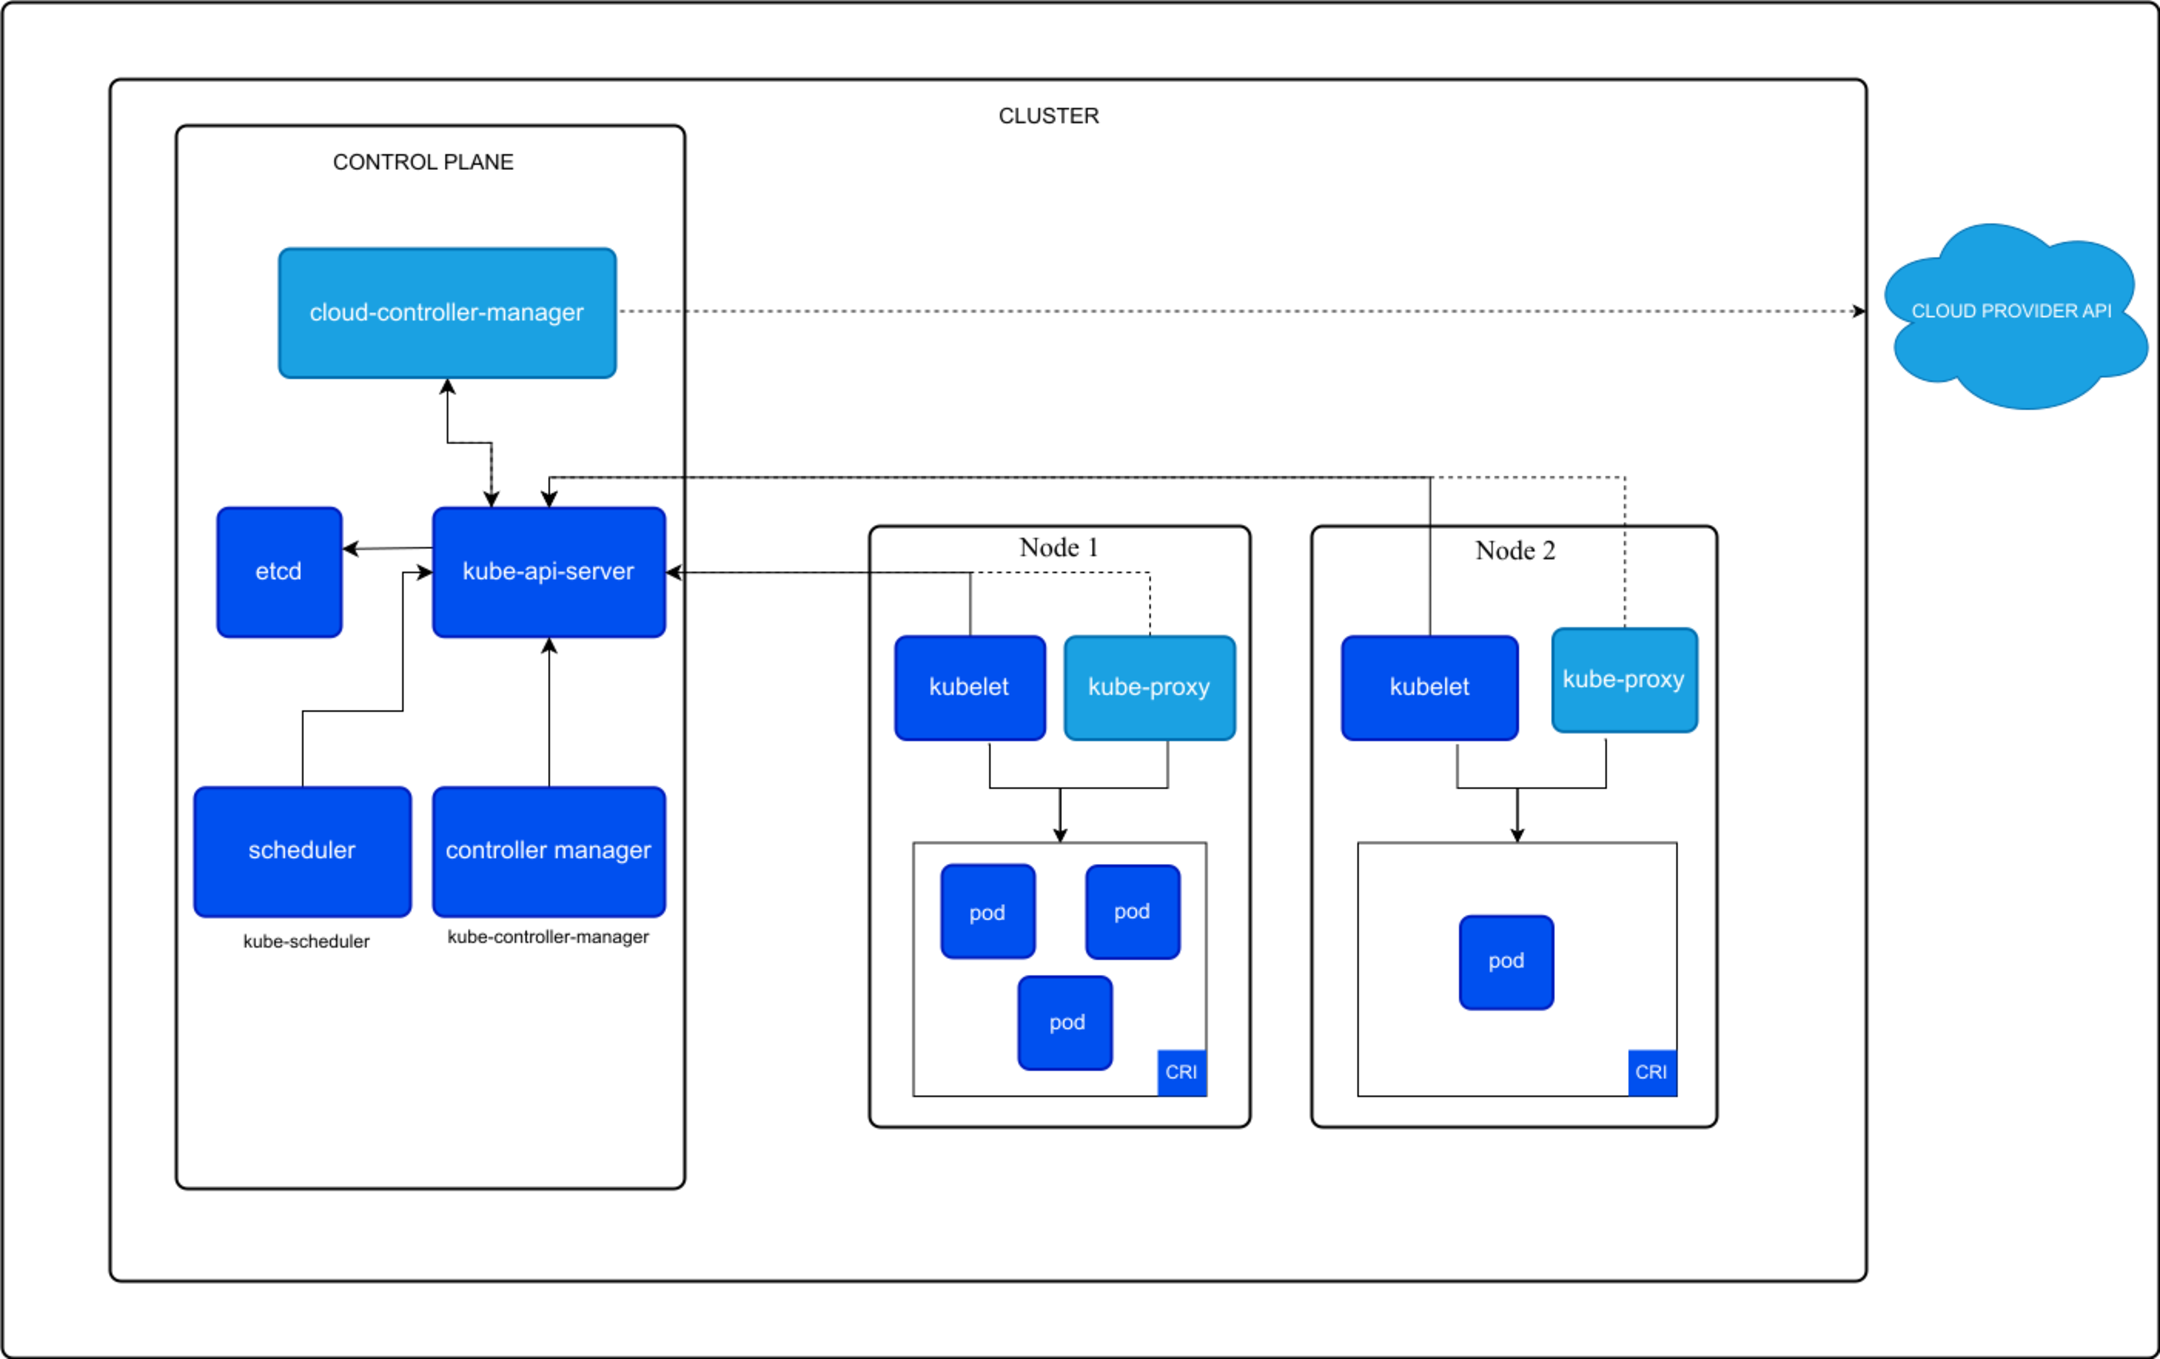
\includegraphics[scale=0.15]{gambar/kubernetes-cluster-architecture.png}

  % Ubah dengan keterangan gambar yang diinginkan
  \caption{Arsitektur Klaster Kubernetes}
  \label{fig:arsitektur-cluster-kubernetes}
\end{figure}

Dalam proses pembuatan klaster Kubernetes, Kubernetes menyediakan \emph{binary} pembantu
yang memudahkan pembuatan bernama kubeadm. Untuk membuat sebuah klaster Kubernetes,
server yang digunakan sebagai \emph{control plane} harus terlebih dahulu menginisiasi
pembuatan klaster. Setelah server \emph{control plane} telah selesai dalam menginisiasi klaster,
server yang digunakan sebagai \emph{worker node} akan digabungkan ke dalam klaster yang sebelumnya
telah dibuat oleh \emph{control plane}. Untuk memudahkan dalam pembuatan klaster, distribusi
Kubernetes bernama K3s akan digunakan dalam implementasi pada tugas akhir ini. Penjelasan
mengenai K3s akan dijelaskan pada bab \ref{chap:K3s}.

\subsubsection{Kubernetes Control Plane}

Pada klaster Kubernetes, server yang menjadi \emph{control plane} bertugas
untuk melakukan \emph{health checking} serta membuat keputusan global seperti \emph{scheduling}
serta mendeteksi dan merespon \emph{event} yang terjadi pada klaster tersebut. Untuk melakukan
tugas tersebut, \emph{control plane} memiliki komponen kube-apiserver,
etcd, kube-scheduler, kube-controller-manager, dan cloud-controller-manager.

\begin{enumerate}
  
  \item Komponen kube-apiserver berperan sebagai antarmuka dari \emph{control plane}.
    Komponen kube-apiserver melayani komunikasi menggunakan operasi RESTful dan
    mengekspos \emph{shared state} dari klaster yang nantinya digunakan untuk
    interaksi antar komponen.

  \item Komponen etcd merupakan tempat penyimpanan \emph{key-value} secara konsisten.
    Komponen etcd digunakan untuk menyimpan semua data pada klaster seperti \emph{state}
    klaster saat ini dan \emph{state} yang diinginkan.

  \item Komponen kube-scheduler merupakan komponen yang mengamati Pod yang telah
    selesai dibuat dan menempatkan Pod ke \emph{node} untuk dijalankan. Pada saat
    menempatkan Pod ke \emph{node}, kube-scheduler memperhitungkan faktor-faktor
    yang berpengaruh seperti batasan \emph{hardware/software}, kebutuhan sumber daya secara
    individu dan kolektif, spesifikasi afinitas dan non-afinitas, \emph{data locality}, interferensi
    antar beban kerja, dan tenggat waktu dari beban kerja.

  \item Komponen kube-controller-manager berperan untuk menjalankan proses \emph{controller}.
    Proses \emph{controller} mengatur komponen sesuai dengan jenis proses \emph{controller},
    salah satu contohnya adalah proses \emph{node controller} yang mengatur jalannya \emph{node}
    seperti mengamati \emph{node} dan merespon ketika \emph{node} mengalami kegagalan.

  \item Komponen cloud-controller-manager merupakan komponen yang berperan sebagai penghubung
    klaster dengan API khusus dari penyedia layanan awan. Komponen ini memisah
    komponen yang berinteraksi dengan penyedia layanan dan komponen yang hanya berinteraksi dengan
    klaster.

\end{enumerate}

\subsubsection{Kubernetes Node}

Pada sebuah klaster Kubernetes, mesin atau server selain \emph{control plane} akan menjadi \emph{worker node}.
\emph{Worker node} bertugas untuk menjalankan Pod. Untuk membantu dalam menjalankan tugas tersebut, komponen \emph{worker node}
memiliki beberapa komponen yaitu kubelet, \emph{container runtime}, dan kube-proxy.

\begin{enumerate}
  
  \item Komponen kubelet merupakan sebuah komponen untuk memastikan \emph{container} berjalan di dalam Pod.
    Komponen kubelet menggunakan konfigurasi dari Podspec yang berupa objek YAML atau JSON yang mendeskripsikan
    sebuah Pod. Komponen kubelet menerima konfigurasi Podspec yang disediakan dari banyak mekanisme seperti
    apiserver dan memastikan bahwa \emph{container} yang didefinisikan pada Podspec berjalan dengan baik. Komponen kubelet
    tidak mengelola \emph{container} yang tidak diciptakan oleh Kubernetes.

  \item Komponen \emph{container runtime} mengelola \emph{container} pada Kubernetes. Komponen \emph{container runtime}
    bertanggung jawab untuk mengelola \emph{container} seperti eksekusi dan siklus hidup dari \emph{container} yang berjalan
    di lingkungan Kubernetes. Kubernetes mendukung \emph{container runtime} yang mengimplementasikan Kubernetes
    CRI (\emph{Container Runtime Interface}).

  \item Komponen kube-proxy mengatur pengaturan jaringan pada setiap \emph{node}. Pengaturan tersebut mengatur komunikasi
    jaringan menuju Pod dari dalam atau luar klaster. Kube-proxy memastikan \emph{request} diteruskan menuju ke
    \emph{container} yang tepat.

\end{enumerate}

\subsection{Objek pada Kubernetes}

Objek pada Kubernetes adalah entitas persisten pada sistem Kubernetes dan digunakan untuk
merepresentasikan keadaan dalam klaster tersebut. Keadaan dalam klaster yang direpresentasikan
oleh objek-objek pada Kubernetes adalah aplikasi yang sedang berjalan pada klaster, \emph{node}
tempat aplikasi berjalan, sumber daya yang tersedia, serta pengaturan kebijakan tentang aplikasi
tersebut.

\subsubsection{Pod}

Pod merupakan unit terkecil yang dapat dibuat dan dikelola pada klaster Kubernetes. Pod sendiri adalah
kumpulan dari satu atau lebih \emph{container} yang berbagi alamat IP dan volume serta
pengaturan mengenai bagaimana \emph{container} tersebut dijalankan. Konfigurasi Pod dapat
diatur dengan konfigurasi deklaratif menggunakan Podspec yang memiliki ekstensi YAML atau JSON.

\subsubsection{Replication Controllers dan ReplicaSet}

Replication Controllers merupakan objek yang mendefinisikan sebuah \emph{pod template}
dan parameter kontrol untuk melakukan \emph{scaling} secara horizontal, yaitu dengan
cara menambahkan atau mengurangi jumlah dari Pod yang sedang berjalan. Replication
Controllers bertanggung jawab untuk memastikan jumlah Pod yang ada pada klaster
sesuai dengan jumlah Pod yang didefinisikan pada konfigurasi.

\subsubsection{Job}

Job merupakan beban kerja pada Kubernetes yang berbasis tugas. Job akan menciptakan
satu atau lebih Pod untuk menyelesaikan tugas Job tersebut. Ketika tugas tersebut
selesai, Pod yang menjalankan tugas tersebut akan berhenti. Job menjamin jumlah
Pod yang diciptakan akan selalu sesuai dengan jumlah Pod yang diinginkan pada
saat menjalankan tugas Job. Ketika sebuah Pod mengalami kegagalan dalam menjalankan
tugas Job, Job dapat menciptakan Pod baru untuk menyelesaikan tugasnya. Job dapat
menciptakan lebih dari satu Pod untuk menjalankan tugas secara paralel.

\subsubsection{Service}

Service merupakan abstraksi dari Pod yang menyediakan alamat IP dan DNS yang
akan digunakan untuk mengakses Pod tersebut. Service pada Kubernetes merupakan
objek yang mengimplementasikan arsitektur REST. Terdapat beberapa tipe dari objek
Service, yaitu ClusterIP, NodePort, LoadBalancer, dan ExternalName.

\begin{enumerate}
  
  \item ClusterIP merupakan tipe dari Service yang melakukan ekspos Service
    pada IP internal klaster. Tipe ClusterIP ini merupakan tipe \emph{default}
    untuk Service. Service yang menggunakan tipe ini hanya dapat diakses di dalam
    klaster saja.

  \item NodePort merupakan tipe dari Service yang melakukan ekspos Service pada alamat IP
    dan \emph{port} statik setiap \emph{node}. NodePort memungkinkan Service untuk diakses dari luar
    dengan melakukan \emph{request} pada NodeIP dan NodePort.

  \item LoadBalancer merupakan tipe dari Service yang mengekspos Service secara eksternal
    menggunakan \emph{load balancer} eksternal. Kubernetes tidak menyediakan komponen
    \emph{load balancing} secara langsung, sehingga komponen \emph{load balancer} harus
    disediakan sendiri oleh pengguna atau pengelola klaster.

  \item ExternalName merupakan tipe dari Service yang memetakan Service dengan \emph{externalName}.
    Hasil pemetakan akan mengkonfigurasi server DNS klaster untuk mengembalikan catatan CNAME dengan
    nilai berupa \emph{externalName} yang sudah dipetakan sebelumnya.

\end{enumerate}

\subsection{K3s}
\label{chap:K3s}

Kubernetes membutuhkan banyak komponen untuk menjalankan platform Kubernetes
seperti etcd sebagai tempat penyimpanan data untuk semua data pada klaster,
\emph{container runtime} sebagai pengelola \emph{container} yang akan
dijalankan pada pods, dan lain-lain. Banyak komponen tersebut terkadang
tidak diperlukan di beberapa skenario. Untuk mengatasi permasalahan tersebut,
sebuah distribusi Kubernetes bernama K3s diciptakan.

K3s \parencite{k3s-website} merupakan distribusi Kubernetes yang diciptakan oleh Rancher Labs yang
memiliki ukuran yang lebih kecil secara keseluruhan. K3s berbentuk
\emph{binary} yang berisi semua \emph{tools} yang dibutuhkan untuk membuat
klaster dan bergabung ke klaster. K3s didesain untuk lingkungan
yang memiliki sumber daya terbatas seperti \emph{edge computing} dan \emph{Internet of Things}.
\emph{Binary} K3s berisi \emph{tools} dan \emph{packages} yang diperlukan untuk membuat
klaster Kubernetes seperti Containerd dan runc sebagai CRI (\emph{Container Runtime Interface}),
Flannel untuk CNI (\emph{Container Network Interface}), CoreDNS untuk Cluster DNS, dan lain-lain.

\subsection{\emph{Container}}
\label{sec:container}

\emph{Container} merupakan sebuah unit perangkat lunak yang ringan yang membungkus
aplikasi dan semua dependensi yang dibutuhkan untuk menjalankan aplikasi tersebut. Dengan menggunakan
\emph{container}, aplikasi yang dibungkus dapat berjalan secara konsisten walaupun dijalankan
di lingkungan yang berbeda.

Pada dasarnya, \emph{container} bisa disebut sebagai produk virtualisasi. Perbedaan
mendasar antara \emph{container} dan \emph{virtual machine} adalah \emph{container}
menggunakan kernel sistem operasi dari \emph{host}, sedangkan \emph{virtual machine} menjalankan
sistem operasi tersendiri secara penuh. Perbedaan tersebut menyebabkan \emph{container} lebih ringan
dibandingkan dengan \emph{virtual machine} sehingga cocok untuk menjalankan aplikasi
yang tidak membutuhkan sistem operasi tersendiri secara penuh.
Untuk menjalankan tugasnya, \emph{container} memiliki beberapa mekanisme/fitur seperti
berikut:

\begin{enumerate}
  
  \item \emph{Namespaces}

    Fitur \emph{namespaces} menyediakan isolasi dengan cara membagi sumber daya sistem
    yang dimiliki oleh \emph{host} seperti PID dan \emph{network interfaces} ke grup
    yang terisolasi. Setiap \emph{container} memiliki \emph{namespace} tersendiri sehingga
    \emph{container} terlihat memiliki sumber daya tersendiri. Hal tersebut mencegah
    adanya konflik dengan \emph{container} lain yang sedang berjalan dalam sistem.

  \item \emph{Control Groups} (cgroups)

    Fitur cgroups digunakan untuk mengalokasi dan membatasi sumber daya seperti CPU, \emph{memory},
    dan \emph{input/output} ke sebuah grup proses. Cgroups memastikan agar \emph{container}
    tidak menggunakan sumber daya \emph{host} secara berlebihan dan memastikan pembagian sumber daya
    secara adil untuk semua \emph{container}.

  \item \emph{UnionFS}

    \emph{UnionFS} adalah jenis dari \emph{filesystem} yang merupakan fitur dari kernel Linux. \emph{Container}
    menggunakan \emph{unionfs} sebagai \emph{filesystem} yang digunakan. Dengan menggunakan
    \emph{unionfs} sebagai \emph{filesystem}, \emph{container} dapat mengatur \emph{disk space}
    dan menangani perubahan yang cepat.

  \item \emph{Container Images}

    \emph{Container images} merupakan sebuah \emph{package} yang bersifat statik yang berisi
    semua dependensi yang dibutuhkan untuk menjalankan aplikasi. \emph{Container images} diciptakan
    melalui serangkaian instruksi dan merupakan \emph{blueprint} dalam menciptakan \emph{container}.
    \emph{Container images} dapat diberi versi dan dapat dibagi, sehingga semua \emph{container}
    yang menggunakan versi tertentu dari \emph{container image} akan bersifat sama.

  \item \emph{Container Runtime}

    Untuk menjalankan \emph{container}, dibutuhkan sebuah \emph{container runtime}. \emph{Container runtime}
    bertanggung jawab atas semua operasi untuk menjalankan \emph{container} seperti mengunduh
    \emph{container images}, membuat sebuah \emph{instance} dari \emph{container}, dan mengatur
    siklus hidup dari \emph{container}.

\end{enumerate}

Kelebihan dari penggunaan \emph{container} adalah sebagai berikut:

\begin{enumerate}

  \item Konsistensi dan Portabilitas

    Mekanisme dasar dari \emph{container} dan \emph{container image} menyebabkan aplikasi
    yang dibungkus ke dalam \emph{container} sudah menjadi satu dengan dependensi-dependensi
    yang diperlukan dalam menjalankan aplikasi. Selain itu, sifat \emph{container image} yang bersifat
    statik dan memiliki versi membuat \emph{container} konsisten dan sangat portabel.

  \item Efisiensi dan Utilisasi Sumber Daya

    Mekanisme \emph{container} yang berbeda dengan \emph{virtual machine} menyebabkan
    \emph{container} lebih ringan dibandingkan dengan \emph{virtual machine}. Jika aplikasi
    tidak memerlukan virtualisasi operasi sistem secara penuh, \emph{container} adalah alternatif
    yang lebih baik secara efisiensi dan utilisasi.

  \item Sifat Isolasi

    Secara \emph{default}, \emph{container} memiliki proses dan sumber daya yang terisolasi, sehingga
    aplikasi yang dijalankan melalui \emph{container} tidak mengganggu \emph{container} lain ataupun
    proses lain yang berjalan di \emph{host}.

\end{enumerate}

\subsection{Podman}
\label{sec:podman}

Podman merupakan salah satu \emph{container engine} selain Docker. Sama seperti Docker,
Podman digunakan untuk mengelola \emph{container} seperti menjalankan \emph{container},
membuat \emph{container}, dan lain-lain. Untuk bisa mengelola \emph{container},
\emph{container engine} seperti Podman dan Docker memerlukan \emph{container runtime} yang \emph{compliat}
dengan OCI (\emph{Open Container Initiative}) seperti runc, crun, dan lain-lain. Podman diciptakan oleh
Red Hat dan bersifat sumber terbuka.

Secara fungsional, Podman sama seperti Docker, namun Podman memiliki beberapa perbedaan seperti berikut:

\begin{enumerate}
  
  \item \emph{Daemonless}

    Tidak seperti Docker yang yang memiliki proses \emph{daemon}, Podman bersifat \emph{daemonless}.
    Proses \emph{daemon} pada Docker dijalankan oleh \emph{root user} sehingga rentan
    terhadap serangan. Dengan mekanisme \emph{daemonless}, \emph{container} dapat dibuat
    secara \emph{rootless} yang lebih aman dibandingkan dengan \emph{rootful}.

  \item \emph{Rootless Containers}

    Podman mendukung penuh untuk menjalankan \emph{container} sebagai pengguna \emph{non-root}.
    Menjalankan \emph{container} sebagai pengguna \emph{non-root} dapat menghindari masalah keamanan
    jika isolasi dari \emph{container} terkompromisasi.

  \item Manajemen \emph{pod}

    Pod merupakan konsep dari Kubernetes berupa kumpulan dari satu atau lebih \emph{container}.
    Kumpulan \emph{container} tersebut saling berbagi sumber daya seperti \emph{network namespaces}
    dan \emph{storage}.

\end{enumerate}

Penggunaan Podman dan Docker tidak berbeda jauh. Podman diciptakan sebagai alternatif Docker.
Podman atau Docker akan digunakan pada implementasi tugas akhir ini untuk membuat \emph{container}
dari aplikasi basis data Postgresql dan Redis. Teori dasar mengenai Postgresql dan Redis akan
dijelaskan pada subbab \ref{sec:postgresql} dan subbab \ref{sec:redis}.

\subsection{Postgresql}
\label{sec:postgresql}

Postgresql merupakan perangkat lunak sistem manajemen basis data relasional
(\emph{Relational Database Management System}/RDBMS) yang bersifat sumber terbuka.
Postgresql menggunakan bahasa SQL (\emph{Structured Query Language}) dalam pengoperasiannya
seperti menambah data, mengambil data, dan menghapus data.

Postgresql memiliki beberapa fitur, yaitu mendukung banyak tipe data seperti \emph{integer} dan
\emph{string}, mendukung integritas data, memiliki performa tinggi dengan \emph{indexing},
mendukung konkurensi dengan menggunakan \emph{Multi-Version Concurrency Control} atau MVCC,
\emph{reliability} dan \emph{disaster recovery} dengan cara replikasi dan \emph{Write-Ahead Logging} atau WAL,
keamanan dengan autentikasi, mendukung ekstensibilitas, dan \emph{internationalisation}.

\subsection{Redis}
\label{sec:redis}

Redis adalah perangkat lunak sumber terbuka basis data dalam memori (\emph{in-memory}).
Redis menawarkan performa tinggi karena setiap data yang disimpan berada di RAM, tidak seperti
perangkat lunak basis data lainnya yang menyimpan data di \emph{disk}.

Redis sebagai perangkat lunak basis data dapat digunakan untuk menyimpan data sama seperti
aplikasi basis data lainnya, namun performa tinggi yang ditawarkan 
dari mekanisme Redis dalam proses penyimpanan digunakan pada beberapa skenario
seperti berikut:

\begin{enumerate}

  \item \emph{Caching}
    
    Proses \emph{caching} adalah proses menyimpan data yang sering diakses ke dalam
    lokasi sementara yang bisa diakses dengan cepat. Dengan menyimpan data yang serin
    diakses ke lokasi yang dapat diakses dengan cepat, proses pengambilan selanjutnya
    dari data tersebut dapat diselesaikan dengan lebih cepat.

  \item \emph{Message Broker/Queue}

    Proses \emph{message broker}/\emph{queue} dapat dianalogikan dengan proses antrian.
    Data dapat dikirimkan dengan \emph{message broker}/\emph{queue} dan konsumer menerima
    data tersebut kemudian menggunakannya untuk melakukan suatu proses.

\end{enumerate}

Redis akan digunakan sebagai basis data antrian \emph{queue} dalam proses \emph{provisioning} dari
\emph{virtual machine}. Antrian tersebut digunakan untuk menghindari konflik dalam proses \emph{provisioning}
lebih dari satu \emph{virtual machine} dalam waktu yang bersamaan.

\subsection{\emph{Multi-tenancy}}
\label{sec:multi-tenancy}

\emph{Multi-tenancy} secara bahasa memiliki arti banyak pengguna atau \emph{tenant}. Dalam konteks
\emph{cloud computing}, \emph{multi tenancy} memiliki definisi pembagian \emph{resource} 
untuk setiap pengguna namun definisi tersebut masih bersifat luas karena implementasi
dari \emph{multi-tenancy} berbeda untuk setiap \emph{service models} \parencite{6830928}.

Pada \emph{service model} yang berupa \emph{Software-as-a-Service} (SaaS), aplikasi
disediakan oleh \emph{Cloud Service Provider} (CSP) berupa jasa. Definisi \emph{multi-tenancy}
pada model ini adalah satu atau lebih pengguna menggunakan aplikasi yang sama tanpa melihat
sumber daya yang digunakan. Pada \emph{service model} yang berupa \emph{Infrastructure-as-a-Service} (IaaS), pengguna
dapat mengatur sendiri infrastruktur yang disediakan oleh CSP seperti \emph{storage resource} dan \emph{network resource}.
Definisi \emph{multi-tenancy} pada model ini adalah dua atau lebih \emph{virtual machine}
yang dimiliki oleh pengguna yang berbeda berada pada satu mesin fisik yang sama.

Dalam implementasi tugas akhir ini, definisi \emph{multi-tenancy} yang digunakan adalah definisi
\emph{multi-tenancy} dalam IaaS, yaitu dua atau lebih \emph{virtual machine} yang dimiliki oleh
pengguna yang berbeda berada pada satu mesin fisik yang sama. Dalam proses \emph{provisioning}, jika
sebuah mesin fisik sudah memiliki \emph{virtual machine} dari pengguna pertama dan
masih memiliki cukup \emph{resource} untuk melayani pengguna lainnya, mesin tersebut
akan membuat \emph{virtual machine} baru untuk pengguna baru tersebut.

\subsection{\emph{Virtual Machine}}
\label{sec:virtual-machine}

\emph{Virtual machine} merupakan lingkungan komputasi terisolasi
yang berjalan di atas mesin fisik. Digagaskan pertama kali oleh IBM
dengan sebuah konsep bernama \emph{time-sharing}. \emph{Time-sharing}
memungkinkan sebuah mesin digunakan oleh lebih dari satu pengguna sehingga
pengguna tersebut terlihat memiliki sebuah mesin tersendiri \parencite{ibm-website}.

\emph{Virtual machine} dikelola oleh hypervisor. Hypervisor bertugas untuk
mengelola \emph{virtual machine} dengan cara mengabstraksi sumber daya perangkat keras
seperti CPU, \emph{memory}, dan penyimpanan dari \emph{host} yang nantinya akan digunakan
oleh \emph{virtual machine}. Hypervisor sendiri terdiri dari beberapa jenis yaitu hypervisor tipe 1
dan hypervisor tipe 2. Perbedaan dari kedua jenis tersebut adalah infrastruktur virtualisasi yang digunakan.
Hypervisor tipe 1 berjalan langsung di atas \emph{hardware} atau biasa disebut \emph{native hypervisor},
sedangkan hypervisor tipe 2 berjalan di atas sistem operasi \parencite{Aalam_2021}. Perbedaan
dari hypervisor tipe 1 dan hypervisor tipe 2 dapat dilihat pada gambar \ref{fig:arsitektur-hypervisor-1-2}.

\begin{figure}[H]
  \centering

  % Ubah dengan nama file gambar dan ukuran yang akan digunakan
  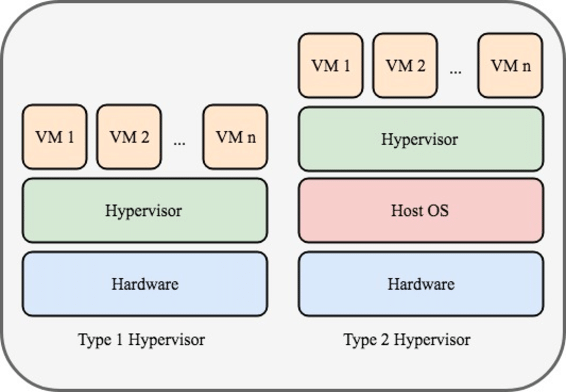
\includegraphics[scale=0.55]{gambar/Type-1-and-type-2-hypervisors.png}

  % Ubah dengan keterangan gambar yang diinginkan
  \caption{Hypervisor Tipe 1 dan Tipe 2 \parencite{nfv}}
  \label{fig:arsitektur-hypervisor-1-2}
\end{figure}

Hypervisor memiliki beberapa fitur untuk mengelola \emph{virtual machine}, yaitu:

\begin{enumerate}
  
  \item Abstraksi sumber daya fisik. Hypervisor menyediakan abstraksi untuk sumber
    daya dari mesin fisik. Abstraksi ini membatasi sumber daya fisik dari mesin yang
    nantinya bisa dipakai oleh \emph{virtual machine}. Dengan abstraksi ini,
    \emph{virtual machine} tidak perlu mengetahui sistem operasi dan \emph{hardware}
    dari \emph{host}.

  \item Isolasi sumber daya fisik. Hypervisor membagi sumber daya fisik dari \emph{host}
    dan membuat entitas terisolasi. Hypervisor memperbolehkan setiap \emph{virtual machine} 
    untuk berjalan secara independen. \emph{Virtual machine} yang terkompromisasi tidak
    akan mengganggu atau membuat \emph{virtual machine} lain juga terkompromisasi. Hal
    tersebut merupakan fungsi dari fitur isolasi sumber daya fisik. Tiap-tiap sumber daya fisik
    yang digunakan oleh \emph{virtual machine} saling terisolasi satu sama lain dan juga
    terisolasi dari sumber daya fisik yang digunakan oleh sistem operasi \emph{host}.

  \item Pengembalian kondisi \emph{virtual machine}. Setiap \emph{virtual machine} menggunakan
    sumber daya fisik dalam bentuk \emph{virtual disk}. \emph{Virtual disk} ini disimpan
    dalam bentuk \emph{file}. \emph{Virtual machine} menyimpan \emph{snapshot} dari \emph{virtual disk}
    dari waktu ke waktu atau setiap ada perubahan dalam \emph{virtual disk} tersebut. Ketika \emph{virtual machine}
    mengalami kendala atau masalah, \emph{virtual machine} dapat dikembalikan ke kondisi \emph{virtual disk}
    yang masih berfungsi sebelumnya.

\end{enumerate}

\subsubsection{QEMU}

QEMU \parencite{qemu-website} adalah emulator dan \emph{virtualizer} mesin generik dan bersifat sumber terbuka.
QEMU dapat digunakan dengan beberapa cara tetapi yang paling umum digunakan adalah sebagai
emulasi sistem. Hasil emulasi sistem tersebut menyediakan model virtual dari sebuah mesin
utuh seperti CPU, memori, dan emulasi perangkat untuk menjalankan sistem operasi \emph{guest}.
Pada mode tersebut, CPU bekerja secara teremulasi sepenuhnya atau dapat bekerja sama
dengan hypervisor seperti KVM, Xen, atau hypervisor lainnya untuk menjalankan sistem
operasi \emph{guest} secara langsung di CPU \emph{host}.
Dalam implementasi tugas akhir ini, QEMU akan digunakan sebagai emulator dan KVM
akan digunakan sebagai hypervisor. Penjelasan mengenai KVM akan dijelaskan pada bab \ref{sec:kvm}.

\subsubsection{KVM}
\label{sec:kvm}

KVM atau \emph{Kernel-based Virtual Machine} \parencite{kvm-website} merupakan \emph{full virtualizer} sumber terbuka
untuk Linux yang memiliki x86 \emph{hardware} dan salah satu hypervisor tipe 1. KVM memiliki ekstensi untuk dua jenis
CPU, yaitu Intel dengan teknologi Intel VT dan AMD dengan teknologi AMD-V. KVM terintegrasi
langsung dengan kernel Linux mulai versi 2.6.20 dengan menyediakan modul kernel kvm.ko yang dapat dimuat.
Modul tersebut menyediakan inti dari infrastruktur untuk virtualisasi. Selain itu, KVM
juga menyediakan modul spesifik untuk Intel yaitu kvm-intel.ko dan untuk AMD yaitu
kvm-amd.ko. Dengan menggunakan KVM, sistem operasi Linux dapat menjalankan satu atau lebih
mesin virtual. Setiap mesin virtual memiliki \emph{hardware} virtual pribadi seperti
\emph{network card}, \emph{disk}, dan \emph{graphics adapter}.

\subsection{Libvirt}
\label{sec:libvirt}

Libvirt adalah \emph{toolkit} sumber terbuka untuk mengelola platform virtualisasi.
Libvirt memudahkan proses pengelolaan platform virtualisasi dengan menyediakan API yang konsisten
dan terstandardisasi untuk banyak jenis hypervisor seperti KVM, QEMU, Xen, VMWare,
dan lain-lain. API tersebut disediakan oleh libvirt sebagai antarmuka interaksi dengan hypervisor.

Libvirt menggunakan arsitektur klien-server, dimana server dari Libvirt berupa daemon
bernama libvirtd yang akan berinteraksi dengan hypervisor yang digunakan dan klien akan
berkomunikasi dengan server atau libvirtd menggunakan protokol yang sudah ditetapkan.
Proses komunikasi antara klien dan server dapat dilakukan dengan beberapa cara, salah
satunya adalah secara terprogram dengan menggunakan bahasa pemrograman.

Libvirt menyediakan \emph{bindings} untuk beberapa bahasa pemrograman seperti Golang, C, Python, dan
lain-lain. Selain itu, Libvirt juga mendukung banyak fitur dari virtualisasi seperti
membuat \emph{virtual machine}, menghentikan \emph{virtual machine} dan menghapus \emph{virtual machine}.

\subsection{\emph{Network Bridge}}
\label{sec:network-bridge}

\emph{Network bridge} merupakan sebuah perangkat yang terdapat pada lapisan ke-dua atau \emph{data link layer} pada
model konseptual OSI atau \emph{Open System Interconnection}. OSI memecah komunikasi jaringan
menjadi tujuh bagian atau lapisan. Model OSI memudahkan berbagai sistem komunikasi
untuk berkomunikasi menggunakan protokol standar.

\emph{Network bridge} menggabungkan dua atau lebih segmen jaringan sehingga terlihat
seperti satu jaringan yang besar. Fungsi dari \emph{network bridge} adalah untuk meneruskan
trafik atau data berdasarkan alamat dari MAC (\emph{Media Access Control}). Tujuan
penggunaan \emph{network bridge} adalah memperluas jaringan lokal atau
membagi jaringan yang lebih besar untuk meningkatkan kinerja dan keamanan \parencite{network-bridge}.

\subsubsection{Linux \emph{Bridge}}

Linux \emph{bridge} adalah salah satu implementasi dari \emph{network bridge} dalam sistem
operasi Linux. Implementasi Linux \emph{bridge} pada kernel Linux sudah
terintegrasi sejak versi 2.4 \parencite{linux-foundation-bridge-website}.
Pada Linux \emph{bridge}, \emph{network bridge} diimplementasikan pada tingkat
perangkat lunak pada kernel Linux. Sama seperti kegunaan dari \emph{network bridge},
Linux \emph{bridge} dapat menyambungkan antarmuka jaringan satu dengan antarmuka jaringan
lainnya yang ada pada sebuah mesin Linux. Visualisasi dari Linux \emph{bridge}
dapat dilihat pada gambar \ref{fig:linux-bridge}

\begin{figure}[H]
  \centering
  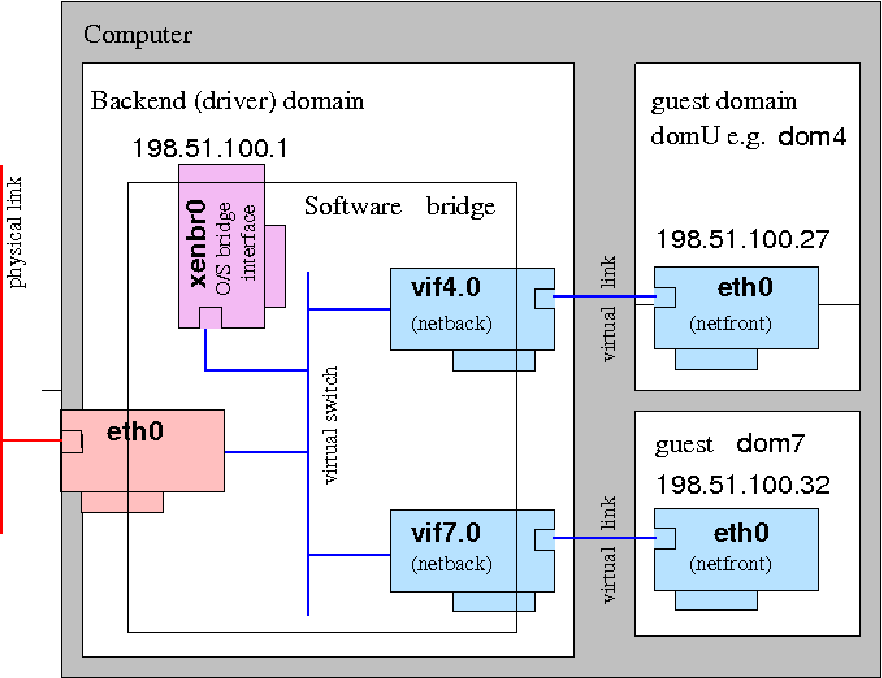
\includegraphics[scale=0.3]{gambar/linux-bridge.png}
  \caption{Visualisasi Linux \emph{Bridge} \parencite{Singh861571}}
  \label{fig:linux-bridge}
\end{figure}

Pada sistem operasi Linux, \emph{Virtual machine} yang dibuat dapat mengutilisasi Linux
\emph{bridge} untuk tersambung dengan jaringan lokal yang sama dengan \emph{host}.
Dengan begitu, alamat IP yang didapat oleh \emph{virtual machine} berada dalam jangkauan
yang sama dengan alamat IP dari \emph{host}, sehingga \emph{virtual machine} tersebut
terlihat sebagai satu mesin fisik tersendiri.

\subsection{RPC}

RPC atau \emph{Remote Procedure Call} adalah sebuah paradigma komunikasi antar program
melalui jaringan internet. RPC memungkinkan sebuah program untuk mengeksekusi sebuah
prosedur atau fungsi yang terdapat pada komputer lain seperti mengeksekusi prosedur
atau fungsi tersebut secara lokal. Konsep mengenai RPC pertama kali dikenalkan oleh
Bruce Jay Nelson melalui disertasinya yang berjudul "Remote Procedure Call" \parencite{rpc}.

Gambaran komunikasi melalui RPC dapat dilihat pada gambar \ref{fig:rpc-communication}.
Pada gambar tersebut, mesin C memanggil prosedur yang terdapat pada mesin S melalui
hubungan internet. Setelah itu, mesin S mengembalikan hasil dari prosedur tersebut
ke mesin C. Hasil prosedur dari mesin S tersebut dapat digunakan oleh
mesin C untuk menjalankan tugasnya tanpa perlu menjalankan prosedur tersebut
secara lokal di mesin C.

\begin{figure}[H]
  \centering
  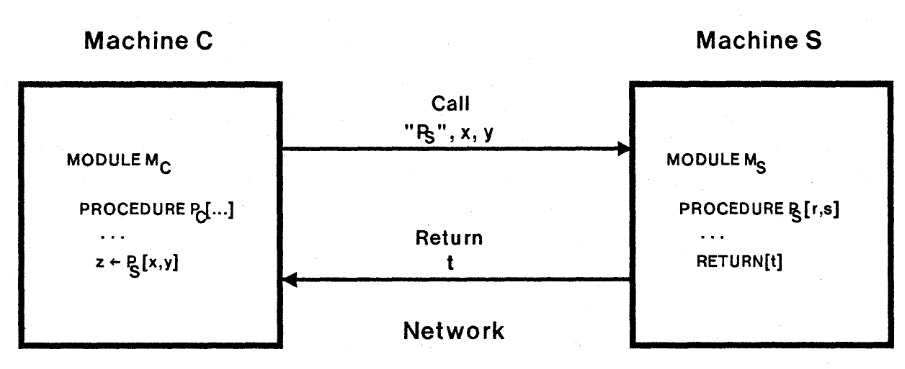
\includegraphics[scale=0.3]{gambar/rpc-communication.png}
  \caption{Komunikasi RPC \parencite{rpc}}
  \label{fig:rpc-communication}
\end{figure}

Gambaran lainnya dari proses RPC terdapat pada gambar \ref{fig:rpc-communication-2}.
Pada gambar tersebut, mesin yang memanggil prosedur atau fungsi melalui RPC memiliki sebuah
\emph{stub} atau \emph{template} dari prosedur atau fungsi yang ingin dipanggil. Mesin
tempat prosedur dipanggil juga memiliki \emph{stub} dari fungsi atau prosedur tersebut namun
mesin tersebut menyediakan \emph{logic} dalam menjalankan fungsi atau prosedur. \emph{Stub}
pada mesin yang memanggil merupakan \emph{identifier} dari fungsi atau prosedur apa yang ingin
dipanggil di mesin tempat fungsi atau prosedur dijalankan.

\begin{figure}[H]
  \centering
  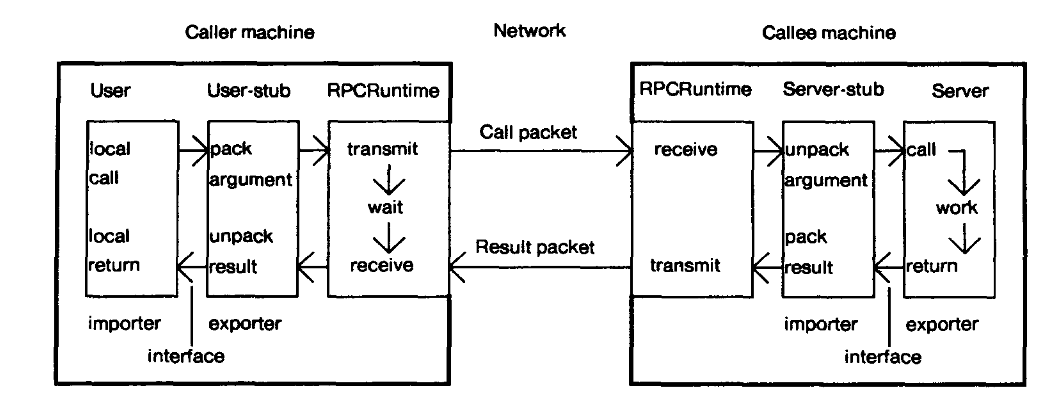
\includegraphics[scale=0.35]{gambar/rpc-communication-2.png}
  \caption{Komunikasi RPC \parencite{implementing-rpc}}
  \label{fig:rpc-communication-2}
\end{figure}

\subsubsection{gRPC}

gRPC adalah implementasi dari RPC yang diciptakan oleh Google. Sama seperti sistem
yang mengimplementasikan sistem RPC, gRPC menggunakan konsep mendefinisikan sebuah \emph{service},
menentukan metode yang bisa dipanggil dari jarak jauh beserta parameter dan tipe data yang
dikembalikan oleh metode tersebut. Secara \emph{default}, gRPC menggunakan protocol buffers
sebagai \emph{Interface Definition Language} (IDL) untuk mendefinisikan antarmuka \emph{service}
dan struktur dari \emph{payload} yang diperlukan oleh \emph{service}. Gambaran garis besar
komunikasi gRPC terdapat pada gambar \ref{fig:grpc-top-level}.

\begin{figure}[H]
  \centering
  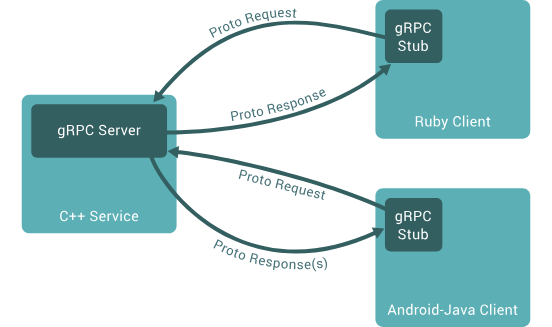
\includegraphics[scale=0.5]{gambar/grpc-usage-image.png}
  \caption{Komunikasi gRPC \parencite{grpc-website-docs-overview}}
  \label{fig:grpc-top-level}
\end{figure}

\subsection{Cloud-init}

Cloud-init merupakan sebuah program sumber terbuka yang berjalan pada saat
\emph{booting} awal dari sebuah \emph{virtual machine} atau \emph{cloud instance}.
Fungsi utama dari Cloud-init adalah untuk menyesuaikan \emph{virtual machine}
atau \emph{cloud instance} dengan data yang diberikan oleh pengguna. Dengan begitu,
setiap \emph{virtual machine} atau \emph{cloud instance} yang dijalankan dengan Cloud-init
akan identik dengan semua konfigurasi yang digunakan. Fungsi tersebut mempermudah dalam 
mengotomisasi konfigurasi awal dari \emph{virtual machine} atau \emph{cloud instance}.

Cloud-init mendukung banyak jenis konfigurasi. Beberapa jenis konfigurasi yang dapat digunakan
pada Cloud-init adalah sebagai berikut:

\begin{enumerate}
  
  \item Antarmuka Jaringan

    Cloud-init dapat mengatur antarmuka jaringan yang digunakan pada \emph{virtual machine}
    atau \emph{cloud instance}. Selain itu, Cloud-init juga dapat menyesuaikan konfigurasi
    antarmuka jaringan tersebut seperti jenis IP, alamat IP, dan lain-lain

  \item \emph{User} dan \emph{Group} Linux

    Selain mengkonfigurasi jaringan, Cloud-init juga mendukung pembuatan \emph{user} dan \emph{group} pada
    sistem operasi Linux pada saat pertama kali \emph{booting}. Konfigurasi lain seperti nama \emph{user},
    nama \emph{group}, \emph{group} dari \emph{user}, dan \emph{password} dari \emph{user} juga didukung
    oleh Cloud-init.

  \item Instalasi \emph{package} dengan \emph{package manager}

    Cloud-init mendukung instalasi \emph{package} menggunakan \emph{package manager} dari distribusi Linux
    seperti Ubuntu. 

  \item \emph{Shell Scripts}

    Cloud-init mendukung penggunaan \emph{shell script} pada saat proses Cloud-init
    berjalan. \emph{Shell scripts} dapat digunakan untuk konfigurasi yang tidak didukung
    oleh Cloud-init seperti menjalankan aplikasi \emph{command line interface} untuk mengunduh
    menggunakan wget dan lain-lain.

\end{enumerate}

\subsection{Golang}

Golang merupakan bahasa pemrograman yang diciptakan oleh Google dan pada 
tahun 2009 dibagi secara publik. \emph{Libraries}
serta fitur-fitur yang ditawarkan oleh Golang seperti \emph{pointer} dan \emph{error as a value}
dapat digunakan dalam banyak kebutuhan seperti pembuatan \emph{services}, \emph{command line interface},
dan lain-lain \parencite{go-website}.

\cleardoublepage

% Bab 3 desain dan implementasi
\chapter{METODOLOGI}
\label{chap:metodologi}

Rancangan implementasi \emph{multi-tenancy} untuk \emph{provisioning}
klaster Kubernetes dimulai dari membuat aplikasi \emph{service} untuk \emph{provisioning}
yang terletak di komputer \emph{worker} untuk membuat
\emph{virtual machine}, kemudian membuat situs web \emph{dashboard} yang nantinya
digunakan oleh \emph{user} untuk membuat klaster Kubernetes secara dinamis dan sewaktu-waktu
menggunakan \emph{virtual machine} yang dibuat oleh aplikasi \emph{provisioning}.
Rancangan tahapan penyelesain implementasi tugas akhir ini
dapat dilihat pada gambar \ref{fig:top-level-implementation}.

\begin{figure}[H]
  \centering
  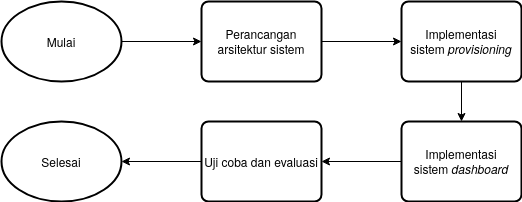
\includegraphics[scale=0.6]{gambar/top-level-implementation.png}
  \caption{Rancangan Penyelesaian Implementasi Tugas Akhir}
  \label{fig:top-level-implementation}
\end{figure}

Berdasarkan gambar \ref{fig:top-level-implementation} di atas, tahapan pertama
dalam rancangan implementasi tugas akhir adalah perancangan arsitektur sistem.
Tahapan perancangan arsitektur sistem berdasarkan kebutuhan sistem yang diperlukan
yaitu situs web sebagai \emph{dashboard} dan aplikasi \emph{provisioning}
untuk membuat \emph{virtual machine}. Setelah perancangan arsitektur sistem telah
selesai, implementasi dari rancangan sebelumnya akan dilakukan. Tahap terakhir
dari tugas akhir ini adalah uji coba dan evaluasi dari sistem yang telah dirancang.
Uji coba dan evaluasi ini bertujuan untuk memeriksa apakah sistem yang telah
diimplementasikan dapat berjalan sesuai kebutuhan dari tugas akhir ini.

\section{Perancangan Arsitektur Sistem}
\label{sec:perancanganarsitektursistem}

Secara garis besar, \emph{workflow} dari implementasi tugas akhir ini dapat dilihat
pada gambar \ref{fig:website-flowchart}. Selain itu, gambaran dari arsitektur sistem
implementasi tugas akhir ini terdapat
pada gambar \ref{fig:server-worker-top-level}. Berdasarkan gambar \ref{fig:server-worker-top-level},
komunikasi antara \emph{worker} dan server utama adalah komunikasi dua arah. Server utama
berkomunikasi dengan \emph{worker} untuk membuat \emph{virtual machine} dan \emph{worker}
berkomunikasi dengan server utama untuk memberi status bahwa \emph{worker} sudah siap
dalam menerima permintaan untuk membuat \emph{virtual machine} serta memberi status dari
pembuatan \emph{virtual machine}.

Setiap komputer fisik yang akan dijadikan \emph{worker} memerlukan aplikasi
atau sebuah \emph{service} yang dapat menerima permintaan pembuatan 
\emph{virtual machine} yang dikirimkan melalui server utama. Selain itu,
server utama juga memerlukan aplikasi yang dapat digunakan oleh pengguna
untuk membuat klaster dengan \emph{virtual machine} pada \emph{worker}.

\begin{figure}[H]
  \centering
  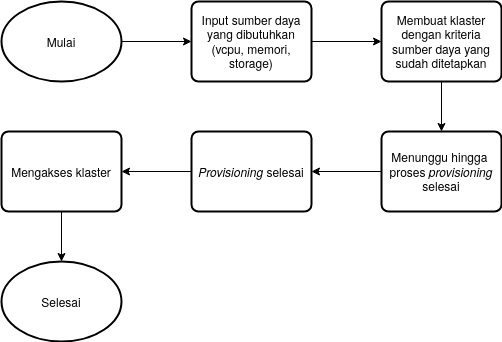
\includegraphics[scale=0.6]{gambar/flowchart-website.png}
  \caption{\emph{Workflow} Penggunaan Aplikasi}
  \label{fig:website-flowchart}
\end{figure}

\begin{figure}[H]
  \centering
  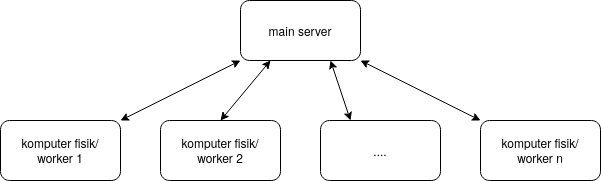
\includegraphics[scale=0.6]{gambar/server-worker-top-level.png}
  \caption{Gambaran Arsitektur Sistem}
  \label{fig:server-worker-top-level}
\end{figure}

\section{Pengembangan Sistem \emph{Provisioning}}
\label{sec:implementasi-sistem-provisioning}

Sistem \emph{provisioning} pada setiap komputer \emph{worker} secara fungsi dapat dipisah
menjadi dua bagian besar, yaitu bagian server untuk menerimaa permintaan pembuatan klaster yang dikirim
oleh server utama dan bagian pembuatan \emph{virtual machine}.

\subsection{Pengembangan Server}
\label{sec:server}

Komputer \emph{worker} menerima \emph{request} pembuatan klaster melalui jaringan internet.
Oleh karena itu, \emph{worker} dapat menerima \emph{request} dengan membuka dan mendengarkan \emph{port}
untuk menerima \emph{request} dari server utama. Implementasi tugas akhir ini menggunakan protokol
RPC dengan gRPC untuk menerima \emph{request} tersebut.

\begin{lstlisting}[
  caption={\emph{Pseudocode} Definisi Prosedur RPC pada Komputer \emph{Worker} Bagian 1},
  label={lst:rpc-procedure-1}
]
PSEUDOCODE_definisi prosedur RPC pada komputer worker

procedure {
  CreateMaster(CreateMasterRequest) returns (CreateMasterResponse) {}
  CreateWorker(CreateWorkerRequest) returns (CreateWorkerResponse) {}
}
\end{lstlisting}

\begin{lstlisting}[
  caption={Definisi Prosedur RPC pada Komputer \emph{Worker} Bagian 2},
  label={lst:rpc-procedure-2}
]
message CreateMasterRequest {
  string cluster_name
  string cluster_token
  number cpu, storage, memory
}

message CreateMasterResponse {
  bool is_success
  string message
  string master_ip_address
  string dashboard_token
}

message CreateWorkerRequest {
  string cluster_name
  string cluster_token
  string master_ip_address
  number cpu, storage, memory
}

message CreateMasterResponse {
  bool is_success
  string message
  string ip_address
  string dashboard_token
}
\end{lstlisting}

Kode sumber \ref{lst:rpc-procedure-1} dan \ref{lst:rpc-procedure-2} menunjukkan fungsi atau prosedur
yang disediakan oleh \emph{worker} menggunakan protokol RPC. Untuk membuat prosedur
di gRPC, format yang dipakai adalah format Protobuf. Protobuf merupakan format
yang digunakan oleh gRPC sebagai \emph{Interface Definition Language}.

Prosedur yang sudah ditulis menggunakan Protobuf akan dikonversi
ke bahasa pemrograman yang diinginkan. Hasil konversi tersebut hanya
berupa fungsi atau prosedur tanpa isi. Isi atau \emph{logic} dari fungsi atau prosedur
tersebut harus dibuat sesuai dengan keinginan pengguna. Hasil konversi dari Protobuf
dapat dibagikan ke komputer lainnya yang memerlukan prosedur tersebut. 

Pada implementasi tugas akhir ini, komputer \emph{worker} menerima
hasil konversi dari prosedur dari Protobuf dan membuat isi dari
prosedur yang sudah ditetapkan. Server utama juga menerima hasil konversi
dan akan menggunakannya untuk menjalankan fungsi atau prosedur tersebut di komputer
\emph{worker}. Isi dari prosedur yang akan dijalankan di komputer \emph{worker} terdapat
pada \emph{pseudocode} \ref{lst:isi-prosedur-1} dan \emph{pseudocode} \ref{lst:isi-prosedur-1}.
Isi prosedur tersebut adalah \emph{logic} untuk membuat \emph{virtual machine} yang berjenis
\emph{master node} atau \emph{worker node}. Perbedaan dari keduanya adalah \emph{master node}
akan bertugas menjadi \emph{control plane} dari klaster Kubernetes yang dibuat nantinya.

\clearpage

\begin{lstlisting}[
  caption={\emph{Pseudocode} Pembuatan \emph{Control Plane} Pada Komputer \emph{Worker}},
  label={lst:isi-prosedur-1}
]
PSEUDOCODE_pembuatan control plane

FUNC CreateMaster
PARAMETER CreateMasterRequest
DO
    LET response BE CreateMasterResponse
    LET instanceRequest BE CreateInstanceRequest
    SET instanceRequest TO CreateMasterRequest

    ADD instanceRequest TO redis.queue
    CALL redis.subscribe WITH request
    
    CASE resultChannel OF
    value:
        SET response TO resultChannel.value
        RETURN response
    ELSE
        RETURN ERROR timeoutExceeded
DONE
\end{lstlisting}

\begin{lstlisting}[
  caption={\emph{Pseudocode} Pembuatan \emph{Worker Node} Pada Komputer \emph{Worker}},
  label={lst:isi-prosedur-2}
]
PSEUDOCODE_pembuatan worker node

FUNC CreateWorker
PARAMETER CreateWorkerRequest
RETURN CreateWorkerResponse 
DO
    LET response BE CreateWorkerResponse
    LET instanceRequest BE CreateInstanceRequest
    SET instanceRequest TO CreateWorkerRequest

    ADD instanceRequest TO redis.queue
    CALL redis.subscribe WITH request
    
    CASE resultChannel OF
    value:
        SET response TO resultChannel.value
        RETURN response
    OTHERS:
        RETURN ERROR timeoutExceeded
DONE
\end{lstlisting}

Komputer \emph{worker} perlu mendengarkan \emph{request} pembuatan melalui
protokol gRPC yang sudah ditetapkan sebelumnya. \emph{Library} gRPC pada Golang
menyediakan API untuk server untuk mendengarkan \emph{request} gRPC di \emph{port}
tertentu. Setelah server mendengarkan di \emph{port} yang telah ditentukan, maka
server tersebut dapat menerima \emph{request} RPC dengan prosedur atau fungsi
yang sudah dibuat melalui \emph{stub}. Kode sumber untuk menjalankan
gRPC server dapat dilihat pada kode sumber \ref{lst:rpc-server-start}.

\clearpage

\begin{lstlisting}[
  caption={Memulai gRPC Server},
  label={lst:rpc-server-start},
]
PSEUDOCODE_menjalankan gRPC server

FUNC StartGrpcServer
DO
    LET listener BE TCP_LISTENER(port)
    LET grpcServer BE GRPC_SERVER

    CALL start_worker
    CALL connect_to_main_server
    CALL grpcServer.serve WITH listener
DONE
\end{lstlisting}

\subsection{Pengembangan Sistem \emph{Provisioning}}
\label{sec:provisioning}

Setelah komputer menerima \emph{request} pembuatan klaster melalui RPC,
\emph{request} tersebut diteruskan ke bagian \emph{provisioning}. Alur 
implementasi \emph{provisioning} dari implementasi ini adalah mempersiapkan
sistem operasi Linux yang akan digunakan sebagai sistem operasi dari
\emph{virtual machine}, mempersiapkan Linux \emph{bridge},
implementasi QEMU dan Libvirt untuk membuat \emph{virtual machine},
implementasi Cloud-init untuk mengkustomisasi \emph{virtual machine}, 
serta implementasi \emph{queue} dan \emph{worker}.
% dan implementasi Websocket untuk \emph{logging}.

\subsubsection{Persiapan Linux untuk \emph{Virtual Machine}}
\label{sec:persiapan-linux-untuk-virtual-machine}

Dalam mempersiapkan sistem operasi Linux yang akan dipakai, terdapat beberapa
hal yang harus dipertimbangkan. Karena \emph{virtual machine} yang akan digunakan
harus siap dengan konfigurasi Cloud-init, maka Linux yang digunakan bukan Linux
yang berbentuk ISO. Linux berbentuk ISO pada saat \emph{booting} akan mengarahkan
\emph{user} untuk proses instalasi sistem operasi Linux dan proses tersebut memerlukan
interaksi dengan pengguna. Selain itu, Linux dalam bentuk ISO tidak memiliki Cloud-init
sehingga tidak memungkinkan untuk menjalankan proses Cloud-init.

Untuk memenuhi kebutuhan tersebut, maka \emph{image} Linux yang digunakan
adalah \emph{image} yang khusus untuk kebutuhan \emph{cloud}. Ubuntu merupakan
salah satu distribusi Linux yang menyediakan \emph{image} khusus tersebut.
Pada implementasi tugas akhir ini, versi Ubuntu yang digunakan adalah Ubuntu 24.10
dengan nama kode "Oracular Oriole". Jenis \emph{file} dari \emph{image} yang akan digunakan
adalah \emph{file} dengan ekstensi .img yang merupakan format \emph{file} untuk \emph{disk image}
yang digunakan oleh QEMU.

Versi Ubuntu yang digunakan pada \emph{cloud image} adalah versi Ubuntu Server yang
berukuran lebih kecil dari \emph{desktop image} dan berisi aplikasi dan \emph{tools}
yang sering digunakan pada server. Namun pada Ubuntu \emph{cloud image}, tidak ada
kata sandi untuk bisa \emph{login} ke \emph{root} pada sistem operasi. Untuk bisa \emph{login},
dibutuhkan kata sandi untuk \emph{root} pada \emph{cloud image} tersebut. Salah satu \emph{tool} yang
dapat digunakan adalah \lstinline{virt-customize}.
Untuk menambahkan kata sandi untuk \emph{root} menggunakan \lstinline{virt-customize} adalah
sebagai berikut:

\begin{lstlisting}[
  style=clistyle,
  caption={\emph{Command} Linux untuk Konfigurasi \emph{Cloud Image}}
]
# virt-customize --add oracular-server-cloudimg-amd64.img --root-password password:root
\end{lstlisting}

Pada \emph{command} di atas, \lstinline{oracular-server-cloudimg-amd64.img} menandakan \emph{file disk image}
mana yang ingin dimodifikasi, \lstinline{--root-password password:root} menandakan bahwa kata sandi
dari \emph{user root} adalah root.

Setelah \emph{user root} sudah memiliki kata sandi, \emph{user root} dapat digunakan
pada Ubuntu tersebut. Pada implementasi tugas akhir ini, modifikasi lain yang dilakukan
terhadap \emph{cloud image} ini adalah mengunduh \emph{binary} dari K3s dan Helm untuk mengurangi
waktu yang dibutuhkan untuk membuat \emph{virtual machine}. Pada implementasi tugas akhir ini,
versi K3s yang digunakan adalah v1.33.1+k3s1 (99d91538) dan versi Helm yang digunakan adalah
v3.18.1 dengan \emph{commit} terakhir f6f87.

\begin{figure}[H]
  \centering
  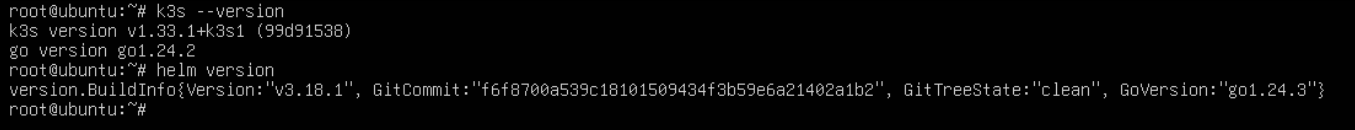
\includegraphics[scale=0.4]{gambar/k3s-helm-version.png}
  \caption{Versi K3s dan Helm}
  \label{fig:k3s-helm-version}
\end{figure}

\emph{Cloud image} Ubuntu secara \emph{default} sudah memiliki Cloud-init. Cloud-init tersebut
tidak perlu dikonfigurasi untuk dapat digunakan. Pada saat \emph{booting virtual machine} untuk yang
pertama kali dengan menggunakan \emph{file} konfigurasi yang diperlukan, Cloud-init akan secara otomatis
menjalankan konfigurasi dari \emph{file} tersebut.

\subsubsection{Persiapan Linux \emph{Bridge}}
\label{sec:persiapan-linux-bridge}

Proses penggabungan \emph{worker node} menggunakan K3s memerlukan alamat IP
dari \emph{control plane}. Karena \emph{virtual machine} yang bertugas menjadi
\emph{worker node} tidak selalu berada di komputer fisik yang sama, sehingga
\emph{control plane} dan \emph{worker node} memerlukan alamat IP di jangkauan
yang sama dengan komputer \emph{host} agar dapat berkomunikasi satu sama lain.
\emph{Virtual machine} dapat memiliki alamat IP di jangkauan yang sama dengan
alamat IP dari \emph{host} menggunakan Linux \emph{bridge}.

Untuk membuat Linux \emph{bridge} di sistem operasi Linux pada implementasi tugas akhir ini,
\emph{tools} NetworkManager akan digunakan. Pemilihan \emph{tools} tersebut karena
NetworkManager merupakan \emph{default tools} yang digunakan pada distribusi Linux
Ubuntu. Selain itu, NetworkManager juga dapat mengatur koneksi internet pada
komputer, termasuk pembuatan Linux \emph{bridge}. Untuk membuat Linux \emph{bridge}
yang bernama k3s-br0 dan \emph{network interface} dari ethernet yang digunakan
adalah enp1s0, dapat menggunakan \emph{command line} sebagai berikut:

\begin{lstlisting}[
  style=clistyle,
  caption={\emph{Command} Linux untuk Konfigurasi Linux \emph{Bridge}},
]
# nmcli con add type bridge ifname k3s-br0 con-name k3s-br0
# nmcli con add type bridge-slave ifname enp1s0 master k3s-br0
# nmcli con down enp1s0
# nmcli con up k3s-br0
\end{lstlisting}

Setelah itu, komputer akan tetap tersambung dengan koneksi internet melalui
\emph{network interface} enp1s0 dan Linux \emph{bridge} k3s-br0 juga aktif.
Linux \emph{bridge} k3s-br0 akan digunakan pada saat membuat \emph{virtual machine}.
\subsubsection{Penggunaan Cloud-init}
\label{sec:implementasi-cloud-init}

Konfigurasi Cloud-init yang digunakan untuk \emph{virtual machine} yang bertugas sebagai \emph{control plane}
dan \emph{worker node} berbeda. Untuk \emph{virtual machine} yang bertugas menjadi \emph{control plane},
ada konfigurasi tambahan dibandingkan dengan \emph{virtual machine} yang bertugas menjadi \emph{worker node}.

\emph{Control plane} dan \emph{worker node} menggunakan konfigurasi jaringan yang sama. \emph{Cloud image}
dari Ubuntu menggunakan \emph{network interface} enp1s0 sebagai \emph{network interface} untuk
koneksi dengan ethernet. Oleh karena itu, \emph{control plane} dan \emph{worker node} menggunakan
konfigurasi jaringan yang sama karena menggunakan \emph{cloud image} yang sama. Kode sumber untuk
konfigurasi jaringan melalui Cloud-init terdapat pada kode sumber \ref{lst:konfigurasi-jaringan}.

\lstinputlisting[
  caption={Konfigurasi Jaringan},
  label={lst:konfigurasi-jaringan},
  style=codestyle,
]{program/cloud-init-network-configuration.yaml}

Pada kode sumber \ref{lst:konfigurasi-jaringan}, sintaks konfigurasi yang dipakai adalah sintaks
konfigurasi versi 2 dari Cloud-init. \emph{Network interface} yang dikonfigurasi adalah \emph{network interface}
enp1s0. \emph{Network interface} tersebut merupakan \emph{default network interface} yang digunakan
oleh \emph{cloud image} Ubuntu untuk jaringan ethernet. Protokol dhcp digunakan agar \emph{virtual machine} mendapatkan
IP secara dinamis dari \emph{host} yang menyediakan Linux \emph{bridge}.

Setelah melakukan konfigurasi jaringan, akan dilakukan konfigurasi lainnya.
Pada \emph{control plane}, konfigurasi lanjutan dari Cloud-init dapat dilihat 
pada kode sumber \ref{lst:konfigurasi-lanjutan-control-plane}.
Untuk \emph{worker node}, konfigurasi lanjutan dari Cloud-init dapat dilihat
pada kode sumber

\begin{lstlisting}[
  caption={Konfigurasi Lanjutan pada \emph{Control Plane} Bagian 1},
  label={lst:konfigurasi-lanjutan-control-plane},
  style=codestyle,
]
#cloud-config
hostname: %s
locale: en_US.UTF-8
timezone: Asia/Jakarta
users:
- default
- name: user
  groups: sudo
  sudo: ALL=(ALL:ALL) ALL
  plain_text_passwd: user
  lock_passwd: false
  shell: /bin/bash

write_files:
- path: /root/service-account.yaml
  content: |
    apiVersion: v1
    kind: ServiceAccount
    metadata:
      name: admin-user
      namespace: kubernetes-dashboard
\end{lstlisting}

\clearpage

\begin{lstlisting}[
  caption={Konfigurasi Lanjutan pada \emph{Control Plane} Bagian 2},
  label={lst:konfigurasi-lanjutan-control-plane-2},
  style=codestyle,
]
- path: /root/role-binding.yaml
  content: |
    apiVersion: rbac.authorization.k8s.io/v1
    kind: ClusterRoleBinding
    metadata:
      name: admin-user
    roleRef:
      apiGroup: rbac.authorization.k8s.io
      kind: ClusterRole
      name: cluster-admin
    subjects:
    - kind: ServiceAccount
      name: admin-user
      namespace: kubernetes-dashboard
- path: /etc/systemd/system/kube-dashboard.service
  content: |
    [Unit]
    Description=Kubernetes dashboard
    Wants=network-online.target
    After=k3s.service

    [Install]
    WantedBy=multi-user.target

    [Service]
    Type=simple
    User=root
    Restart=always
    RestartSec=5s
    ExecStart=/usr/local/bin/k3s \
        kubectl -n kubernetes-dashboard \
        port-forward svc/kubernetes-dashboard-kong-proxy \
        8443:443 --address 0.0.0.0 \

runcmd:
- |
  echo "running command"
  echo "updating and upgrading packages"
  echo "installing necessary packages"

  echo "installing k3s"
  curl -sfL https://get.k3s.io | INSTALL_K3S_SKIP_DOWNLOAD=true INSTALL_K3S_EXEC="server --token %s" sh -s -

  export KUBECONFIG=/etc/rancher/k3s/k3s.yaml
  echo "export KUBECONFIG=/etc/rancher/k3s/k3s.yaml" >> /etc/profile

  echo "creating kubernetes dashboard"
  helm repo add kubernetes-dashboard https://kubernetes.github.io/dashboard/
\end{lstlisting}

\clearpage

\begin{lstlisting}[
  caption={Konfigurasi Lanjutan pada \emph{Control Plane} Bagian 3},
  label={lst:konfigurasi-lanjutan-control-plane-3},
  style=codestyle,
]
  helm upgrade --install kubernetes-dashboard kubernetes-dashboard/kubernetes-dashboard --create-namespace --namespace kubernetes-dashboard
  echo "setting up user for kubernetes dashboard"
  k3s kubectl apply -f /root/service-account.yaml -f /root/role-binding.yaml

  echo "writing token and starting the dashboard..."
  echo "waiting until all pods in the kubernetes-dashboard namespaces is running"
  k3s kubectl wait pod --all --for=condition=Ready --namespace=kubernetes-dashboard --timeout=-1s
  systemctl start kube-dashboard.service

  echo "done"
\end{lstlisting}

Kode sumber \ref{lst:konfigurasi-lanjutan-control-plane}-\ref{lst:konfigurasi-lanjutan-control-plane-3}
mengkonfigurasi beberapa hal pada \emph{control plane} seperti berikut:

\begin{enumerate}
  
  \item \lstinline{hostname} menentukan nama \emph{hostname} pada \emph{virtual machine}.
    Konfigurasi Cloud-init akan digunakan pada bahasa Golang sehingga \lstinline{%s}
    akan dipakai karena penentuan nama \emph{hostname} dilakukan secara dinamis.

  \item \lstinline{locale} menentukan \emph{locale} yang akan dipakai.

  \item \lstinline{timezone} menentukan waktu yang dipakai yaitu Waktu Indonesia Barat (WIB)

  \item \lstinline{users} menandakan konfigurasi \emph{user} yang akan digunakan. Pada
    contoh tersebut, terdapat dua \emph{user} yang akan dibuat pada \emph{virtual machine},
    yaitu \emph{user default} dan \emph{user} dengan nama user. \emph{User default} merupakan
    \emph{user} admin bawaan.

  \item \lstinline{write_files} berisi \emph{file} apa saja yang akan dibuat beserta konten
    dari \emph{file} tersebut. Pada contoh kode sumber, terdapat 3 \emph{file} yang akan dituliskan.
    \emph{File} pertama adalah \emph{file} berekstensi yaml yang akan digunakan untuk membuat
    ServiceAccount pada klaster Kubernetes. \emph{File} selanjutnya adalah \emph{file} berekstensi
    yaml yang akan digunakan untuk RoleBinding ke ServiceAccount yang dibuat menggunakan
    \emph{file} pertama. \emph{File} terakhir merupakan \emph{file} konfigurasi 
    \emph{service} systemd untuk \emph{dashboard} Kubernetes.

  \item \lstinline{runcmd} merupakan daftar dari \emph{command line} yang akan dijalankan.
    \emph{Command line} yang akan dijalankan adalah \emph{command line} untuk membuat klaster
    Kubernetes menggunakan K3s, menambahkan Repository Helm kubernetes-dashboard ke dalam
    klaster Kubernetes, menggunakan \emph{file} untuk klaster Kubernetes yang sudah dibuat
    melalui \lstinline{write_files}, serta menjalankan \emph{service} systemd untuk
    kubernetes-dashboard.

\end{enumerate}

\begin{lstlisting}[
  style=codestyle,
  caption={Konfigurasi Lanjutan pada \emph{Worker Node} Bagian 1},
  label={lst:konfigurasi-lanjutan-worker-node},
]
#cloud-config
hostname: %s
locale: en_US.UTF-8
timezone: Asia/Jakarta
users:
- default
\end{lstlisting}

\clearpage

\begin{lstlisting}[
  style=codestyle,
  caption={Konfigurasi Lanjutan pada \emph{Worker Node} Bagian 2},
  label={lst:konfigurasi-lanjutan-worker-node-2},
]
- name: user
  groups: sudo
  sudo: ALL=(ALL:ALL) ALL
  plain_text_passwd: user
  lock_passwd: false
  shell: /bin/bash

runcmd:
- echo "installing k3s"
- curl -sfL https://get.k3s.io | INSTALL_K3S_SKIP_DOWNLOAD=true INSTALL_K3S_EXEC="agent --server https://%s:6443 --token %s" sh -s -
- echo "done"
\end{lstlisting}

Kode sumber \ref{lst:konfigurasi-lanjutan-worker-node}-\ref{lst:konfigurasi-lanjutan-worker-node-2}
mengkonfigurasi beberapa hal pada \emph{worker node} seperti berikut:

\begin{enumerate}
  
  \item \lstinline{hostname} menentukan nama \emph{hostname} pada \emph{virtual machine}.
    Konfigurasi Cloud-init akan digunakan pada bahasa Golang sehingga \lstinline{%s}
    akan dipakai karena penentuan nama \emph{hostname} dilakukan secara dinamis.

  \item \lstinline{locale} menentukan \emph{locale} yang akan dipakai.

  \item \lstinline{timezone} menentukan waktu yang dipakai yaitu Waktu Indonesia Barat (WIB)

  \item \lstinline{users} menandakan konfigurasi \emph{user} yang akan digunakan. Pada
    contoh tersebut, terdapat dua \emph{user} yang akan dibuat pada \emph{virtual machine},
    yaitu \emph{user default} dan \emph{user} dengan nama user. \emph{User default} merupakan
    \emph{user} admin bawaan.

  \item \lstinline{runcmd} merupakan daftar dari \emph{command line} yang akan dijalankan.
    \emph{Command line} yang akan dijalankan adalah \emph{command line} untuk bergabung ke
    klaster Kubernetes yang dibuat oleh \emph{control plane} menggunakan K3s.

\end{enumerate}

\subsubsection{Penggunaan \emph{Queue} dan \emph{Worker}}
\label{sec:implementasi-queue-dan-worker}

Mekanisme \emph{queue} akan digunakan pada saat proses \emph{provisioning}
\emph{virtual machine} untuk menghindari permasalahan yang dapat muncul ketika
lebih dari satu \emph{virtual machine} dibuat secara bersamaan. \emph{Queue}
akan berisi permintaan serta parameter yang dibutuhkan untuk membuat
\emph{virtual machine}. Untuk mengerjakan permintaan tersebut, sistem \emph{worker}
akan digunakan.

Redis akan digunakan dalam mengimplementasikan mekanisme \emph{queue}. Redis mendukung
penggunaan basis data dalam bentuk \emph{queue} yang bersifat \emph{First In First Out}.
Pada struktur data \emph{queue}, dua operasi utama yang dibutuhkan adalah penambahan data
ke \emph{queue} dan pengambilan data dari \emph{queue}. Kode sumber penambahan data \emph{queue}
dan pengambilan data dari \emph{queue} dapat dilihat pada kode sumber
\ref{lst:penambahan-data-ke-queue} dan \ref{lst:pengambilan-data-dari-queue}.

\begin{lstlisting}[
  style=codestyle,
  caption={Operasi Penambahan Data ke \emph{Queue}},
  label={lst:penambahan-data-ke-queue},
]
PSEUDOCODE_penambahan data ke queue
FUNC AddToQueue
PARAM CreateInstanceRequest
DO
    CALL redis.leftPush WITH CreateInstanceRequest
DONE
\end{lstlisting}

\clearpage

\begin{lstlisting}[
  style=codestyle,
  caption={Operasi Pengambilan Data dari \emph{Queue}},
  label={lst:pengambilan-data-dari-queue},
]
PSEUDOCODE_pengambilan data dari queue

FUNC PopQueue
RETURN CreateInstanceRequest
DO
    LET queue BE ThisComputerProvisioningQueue
    LET result BE CreateInstanceRequest

    LET data BE CALL redis.rightPop
    SET result TO data

    RETURN result
DONE
\end{lstlisting}

Selain itu, Redis juga dapat digunakan sebagai implementasi dari paradigma \emph{message delivery}
dalam bentuk \emph{publisher} dan \emph{subscriber}. Subjek yang menjadi
\emph{subscribe} dapat menunggu pesan dalam sebuah \emph{channel} dan 
\emph{publisher} dapat mengirim pesan ke dalam \emph{channel} tersebut.
Pada implementasi tugas akhir ini, \emph{message delivery} digunakan
sebagai bentuk komunikasi antara \emph{worker} dengan sistem \emph{provisioning}.
Sistem komunikasi tersebut bertujuan agar \emph{worker} dapat menerima hasil
dari \emph{provisioning}. Kode sumber fungsi \emph{publisher} dan \emph{subscriber}
pada \emph{queue} dapat dilihat pada kode sumber \ref{lst:queue-pub} dan \ref{lst:queue-sub}.

\begin{lstlisting}[
  caption={Operasi \emph{Publisher}},
  label={lst:queue-pub},
  style=codestyle,
]
PSEUDOCODE_publisher

FUNC Publish
PARAM channel, message
DO
    CALL redis.publish WITH channel, message
DONE
\end{lstlisting}

\begin{lstlisting}[
  caption={Operasi \emph{Subscriber}},
  label={lst:queue-sub},
  style=codestyle,
]
PSEUDOCODE_subscriber

FUNC Subscribe
PARAM channel
DO
    CALL redis.subscribe WITH channel
DONE
\end{lstlisting}

\emph{Worker} digunakan untuk menjalankan tugas \emph{provisioning}
yang terdapat pada \emph{queue}. \emph{Worker} akan diimplementasikan
sebagai sebuah goroutine menggunakan bahasa pemrograman Golang. Goroutine merupakan
fitur pada bahasa pemrograman untuk menjalankan sebuah fungsi atau proses
di \emph{background} sehingga tidak terjadi situasi \emph{blocking}. Kode sumber
fungsi \emph{worker} dapat dilihat pada kode sumber \ref{lst:fungsi-worker}.

\clearpage

\begin{lstlisting}[
  caption={Fungsi pada \emph{Worker}},
  label={lst:fungsi-worker},
  style=codestyle,
]
PSEUDOCODE_fungsi worker

FUNC DoWork
DO
    WHILE TRUE
    DO
        LET instanceRequest BE CALL PopQueue
        LET res BE CALL CreateInstance with instanceRequest
        CALL Publish WITH instanceRequest.name, res
    DONE
DONE
\end{lstlisting}

Pada kode sumber \ref{lst:fungsi-worker}, \emph{worker} memanggil fungsi
dari \emph{queue} yaitu fungsi untuk mengambil data dari \emph{queue}
di dalam sebuah \emph{loop} yang tidak akan pernah selesai. Setelah
mendapatkan data permintaan dan parameter yang dibutuhkan untuk \emph{provisioning},
permintaan dan parameter diteruskan ke fungsi untuk membuat \emph{instance}
dari \emph{virtual machine}.

% \subsubsection{Implementasi Websocket}
% \label{sec:implementasi-websocket}
%
% Untuk menunjukkan proses dalam pembuatan \emph{virtual machine}

\subsubsection{Penggunaan QEMU dan Libvirt}
\label{sec:implementasi-libvirt}

Libvirt menyediakan \emph{bindings} untuk banyak bahasa pemrograman
untuk berkomunikasi dengan Libvirt. Libvirt juga menyediakan API untuk
mengelola \emph{virtual machine} dan teknologi virtualisasi.

Dalam implementasi tugas akhir ini, QEMU dan Libvirt akan digunakan.
Untuk menggunakan QEMU sebagai emulator dan interaksi dengan QEMU menggunakan Libvirt,
Libvirt memerlukan konfigurasi koneksi dengan QEMU. Kode sumber untuk konfigurasi
tersebut dapat dilihat pada kode sumber \ref{lst:konfigurasi-qemu-libvirt}.

\begin{lstlisting}[
  caption={Konfigurasi QEMU dengan Libvirt},
  label={lst:konfigurasi-qemu-libvirt},
  style=codestyle,
]
PSEUDOCODE_konfigurasi koneksi dengan Libvirt

FUNC InitLibvirtConnection
RETURN LibvirtConnection
DO
    LET conn BE CALL libvirt.NewConnection WITH "qemu://system"

    RETURN conn
DONE
\end{lstlisting}

Pada kode sumber \ref{lst:konfigurasi-qemu-libvirt}, \lstinline{qemu:///system} akan
digunakan sebagai koneksi ke \emph{daemon} dari Libvirt yang berjalan sebagai \emph{root}.
Koneksi tersebut akan digunakan untuk komunikasi antara \emph{bindings} dari Libvirt yang
dipakai dengan teknologi virtualisasi QEMU.

Proses \emph{provisioning} menggunakan Libvirt terdiri dari beberapa langkah, yaitu:

\begin{enumerate}

  \item Membuat \emph{file} konfigurasi untuk Cloud-init

    Untuk menggunakan Cloud-init dengan konfigurasi yang diinginkan, \emph{file}
    yang berisi konfigurasi Cloud-init harus diubah menjadi \emph{disk} dan digunakan
    pada saat membuat \emph{virtual machine}. Kode sumber untuk membuat \emph{file}
    konfigurasi jaringan terdapat pada kode sumber \ref{lst:pembuatan-file-konfigurasi-jaringan}.

    \begin{lstlisting}[
      caption={Pembuatan \emph{File} Konfigurasi Jaringan},
      label={lst:pembuatan-file-konfigurasi-jaringan},
      style=codestyle,
    ]
PSEUDOCODE_pembuatan file Cloud-init untuk konfigurasi jaringan

FUNC CreateNetwork
DO
    LET networkConfiguration BE CloudNetworkConfiguration

    CALL WriteFile WITH networkConfiguration
DONE
    \end{lstlisting}

    Setelah \emph{file} konfigurasi jaringan telah dibuat, \emph{file}
    konfigurasi lanjutan untuk Cloud-init akan dibuat. Kode sumber untuk membuat
    \emph{file} konfigurasi lanjutan \emph{virtual machine} yang bertugas
    menjadi \emph{control plane} dan \emph{worker node} terdapat pada kode sumber
    \ref{lst:pembuatan-file-konfigurasi-control-plane} dan \ref{lst:pembuatan-file-konfigurasi-worker-node}.

    \begin{lstlisting}[
      caption={Pembuatan \emph{File} Konfigurasi Lanjutan \emph{Control Plane}},
      label={lst:pembuatan-file-konfigurasi-control-plane},
      style=codestyle,
    ]
PSEUDOCODE_pembuatan file Cloud-init untuk Control Plane

FUNC CreateControlPlaneCloudInit
DO
    LET configuration BE ControlPlaneConfiguration
    LET networkConfiguration BE CloudNetworkConfiguration
    
    CALL WriteFile WITH configuration
    CALL cloud-localds WITH configuration, networkConfiguration
DONE
    \end{lstlisting}

    \begin{lstlisting}[
      caption={Pembuatan \emph{File} Konfigurasi Lanjutan \emph{Worker Node}},
      label={lst:pembuatan-file-konfigurasi-worker-node},
      style=codestyle,
    ]
PSEUDOCODE_pembuatan file Cloud-init untuk Worker Node

FUNC CreateWorkerNodeCloudInit
DO
    LET configuration BE WorkerNodeConfiguration
    LET networkConfiguration BE CloudNetworkConfiguration
    
    CALL WriteFile WITH configuration
    CALL cloud-localds WITH configuration, networkConfiguration
DONE
    \end{lstlisting}

    Pada kode sumber \ref{lst:pembuatan-file-konfigurasi-control-plane}
    dan \ref{lst:pembuatan-file-konfigurasi-worker-node}, \emph{disk}
    dibuat menggunakan \emph{tool} \lstinline{cloud-localds}. \emph{Tool}
    tersebut menghasilkan \emph{file} berekstensi iso yang nantinya akan
    dipasangkan ke \emph{virtual machine}.

  \item Menyalin \emph{cloud image}

    \emph{Cloud image} yang sudah dimodifikasi sebelumnya disalin untuk
    setiap \emph{virtual machine} yang akan dibuat dan dilakukan proses
    \emph{resize} sesuai dengan ukuran penyimpanan yang diinginkan oleh
    pengguna. Kode sumber untuk menyalin dan melakukan proses \emph{resize}
    terdapat pada kode sumber \ref{lst:penyalinan-cloud-image}

    \clearpage

    \begin{lstlisting}[
      caption={Penyalinan \emph{cloud image}},
      label={lst:penyalinan-cloud-image},
      style=codestyle,
    ]
PSEUDOCODE_penyalinan cloud image

FUNC CopyImage
PARAM instanceName, instanceConfig
DO
    LET data BE CALL ReadFile WITH baseImage
    LET destinationPath BE image_dir + "/" + instanceName

    CALL WriteFile WITH destinationPath, data
    CALL ResizeImage WITH instanceConfig.Storage
DONE
    \end{lstlisting}

  \item Membuat \emph{virtual machine}

    Untuk membuat \emph{virtual machine} melalui Libvirt, konfigurasi
    mengenai \emph{virtual machine} tersebut perlu diberikan. Libvirt menggunakan
    \emph{file} berekstensi xml untuk konfigurasi \emph{virtual machine}.
    Kode sumber untuk mengatur konfigurasi xml \emph{virtual machine} terdapat
    pada kode sumber \ref{lst:konfigurasi-xml-virtual-machine}

    \begin{lstlisting}[
      caption={Konfigurasi xml \emph{Virtual Machine}},
      label={lst:konfigurasi-xml-virtual-machine},
      style=codestyle,
    ]
PSEUDOCODE_pengaturan konfigurasi xml virtual machine

FUNC CreateVirtualMachineXml
PARAM instanceName, instanceConfig
RETURN string
DO
    LET instanceIso BE image_dir + "/" + instanceName
    LET cloudConfig BE cloud_config_dir + "/" + instanceName
    LET xmlConfig BE libvirtXml WITH instanceIso, cloudConfig

    RETURN xmlConfig
DONE
    \end{lstlisting}

    Setelah konfigurasi xml dari \emph{virtual machine} telah dibuat, Libvirt
    dapat menggunakan konfigurasi tersebut untuk membuat \emph{virtual machine}.
    Kode sumber untuk membuat \emph{virtual machine} menggunakan konfigurasi
    xml dapat dilihat pada kode sumber \ref{lst:pembuatan-vm}.

    \begin{lstlisting}[
      caption={Pembuatan \emph{Virtual Machine}},
      label={lst:pembuatan-vm},
      style=codestyle,
    ]
PSEUDOCODE_pembuatan virtual machine

FUNC CreateVirtualMachine
PARAM instanceRequest
RETURN 
DO
    LET instanceName BE random_string
    LET conn BE CALL InitLibvirtConnection

    CALL CreateNetwork
    LET configuration BE CALL CreateVMCloudInit
    CALL CopyImage WITH instanceName, instanceRequest
    CALL conn.CreateVM WITH configuration
DONE
    \end{lstlisting}

  \item Menunggu proses Cloud-init

    Cloud-init memerlukan beberapa waktu untuk menyelesaikan tugasnya.
    Beberapa proses memerlukan proses yang dijalankan oleh Cloud-init
    untuk selesai terlebih dahulu. Untuk menunggu proses Cloud-init selesai,
    ditunjukkan pada kode sumber \ref{lst:menunggu-cloud-init}.

    \begin{lstlisting}[
      caption={Menunggu Proses Cloud-init Selesai},
      label={lst:menunggu-cloud-init},
      style=codestyle,
    ]
PSEUDOCODE_menunggu proses Cloud-init selesai

FUNC WaitCloudInit
PARAM instanceRequest
DO
    LET dom BE VMDomain
    LET waitCloudInit BE "cloud-init status --wait"
    CALL dom.QemuAgentCommand WITH waitCloudInit
DONE
    \end{lstlisting}

\end{enumerate}

\section{Implementasi Situs Web}
\label{sec:implementas-situs-web}

Situs web yang dibuat akan digunakan sebagai pengguna untuk membuat
klaster Kubernetes menggunakan \emph{virtual machine} yang dibuat
oleh sistem \emph{provisioning}. Implementasi situs web dibagi menjadi
dua yaitu implementasi bagian \emph{frontend} dan bagian \emph{backend}.

\subsection{Implementasi \emph{Frontend}}
\label{subsec:implementas-frontend}

Situs web \emph{dashboard} merupakan antarmuka yang akan digunakan oleh \emph{user}
untuk membuat klaster Kubernetes. Pada situs web tersebut, terdapat
informasi mengenai identitas komputer yang siap
menerima permintaan untuk membuat \emph{virtual machine}.
Tampilan dari \emph{dashboard} dapat dilihat pada gambar
dan \ref{fig:dashboard-with-node}.

\begin{figure}[H]
  \centering
  \fbox{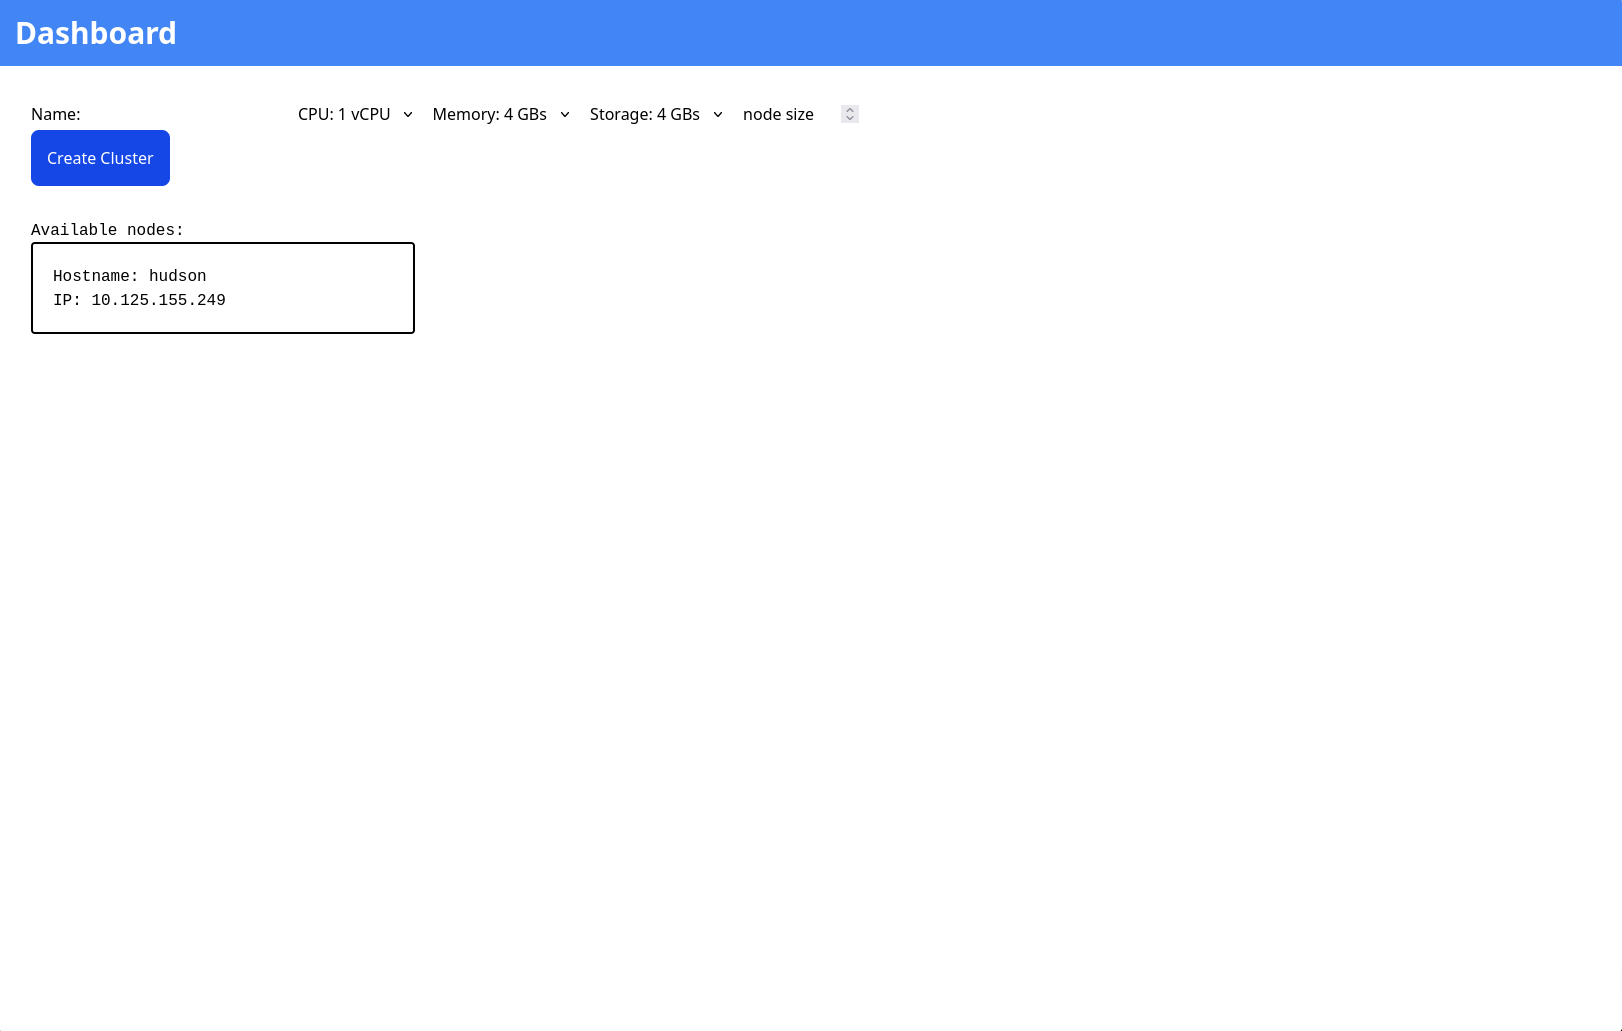
\includegraphics[scale=0.3]{gambar/dashboard-with-node.png}}
  \caption{Tampilan \emph{Dashboard}}
  \label{fig:dashboard-with-node}
\end{figure}

Pada contoh gambar \ref{fig:dashboard-with-node}, terdapat satu komputer \emph{worker}
yang siap untuk menerima permintaan, yaitu komputer yang memiliki \emph{hostname} hudson dan alamat
ip 10.125.155.249.

% TODO: implementasi backend
\subsection{Implementasi \emph{Backend}}
\label{subsec:implementas-backend}

Bagian \emph{backend} dari situs web bertanggung jawab untuk menangani permintaan
yang dibuat pengguna pada bagian \emph{frontend}. Selain itu, bagian \emph{backend}
juga bertanggung jawab untuk melakukan komunikasi dengan komputer \emph{worker} menggunakan
protokol RPC melalui gRPC. Garis besar pertukaran informasi dan komunikasi
dapat dilihat pada gambar \ref{fig:frontend-backend-worker}.

\begin{figure}[H]
  \centering
  \fbox{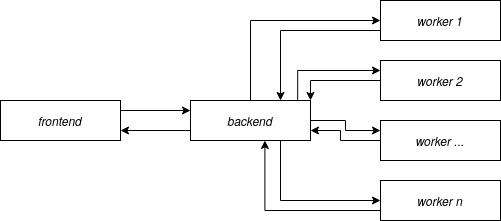
\includegraphics[scale=0.55]{gambar/frontend-backend-worker.png}}
  \caption{Komunikasi \emph{Frontend-Backend-Worker}}
  \label{fig:frontend-backend-worker}
\end{figure}

\cleardoublepage

% Bab 4 pengujian dan analisis
\chapter{HASIL DAN PEMBAHASAN}
\label{chap:hasil-pembahasan}

Pada bab ini akan dijelaskan mengenai hasil implementasi
dan pengujian dari sistem \emph{provisioning} yang telah
dibuat sebelumnya pada bab 3. Pengujian yang dilakukan
menggunakan laptop penulis dan komputer dari laboratorium Rekayasa Perangkat
Lunak Teknik Informatika ITS. Spesifikasi dari laptop dan komputer
yang digunakan dapat dilihat pada tabel \ref{tb:spesifikasi-laptop-pengujian} dan
\ref{tb:spesifikasi-komputer-pengujian}

\begin{longtable}{|c|c|}
  \caption{Spesifikasi Laptop untuk Pengujian}
  \label{tb:spesifikasi-laptop-pengujian} \\
  \hline
  OS     & Fedora Linux 42.20250614.0 (Kinoite) x86\_64 \\
  \hline
  Kernel & Linux 6.14.9-300.fc42.x86\_64                \\
  \hline
  CPU    & Intel(R) Core(TM) i7-10750H (12) @ 5.00 GHz       \\
  \hline
  Integrated GPU   & Intel UHD Graphics @ 1.15 GHz [Integrated]       \\
  \hline
  Discrete GPU    & NVIDIA GeForce GTX 1650 Ti Mobile [Discrete]       \\
  \hline
  RAM    & 15848MiB       \\
  \hline
\end{longtable}

\begin{longtable}{|c|c|}
  \caption{Spesifikasi Komputer untuk Pengujian}
  \label{tb:spesifikasi-komputer-pengujian} \\
  \hline
  OS     & Ubuntu 24.04.2 LTS x86\_64 \\
  \hline
  Kernel & 6.11.0-26-generic          \\
  \hline
  CPU    & 12th Gen Intel i7-12700 (20) @ 4.800GHz       \\
  \hline
  GPU    & Intel AlderLake-S GT1       \\
  \hline
  RAM    & 31834MiB       \\
  \hline
\end{longtable}

\section{Hasil Implementasi}
\label{sec:hasil-implementasi}

\subsection{Implementasi Linux Bridge}
\label{subsec:implementasi-linux-bridge}

Linux \emph{bridge} yang telah dijelaskan sebelumnya dibuat
agar \emph{virtual machine} memiliki jangkauan alamat IP yang sama
dengan jangkauan alamat IP dari komputer \emph{host}. Jangkauan IP yang
sama dengan komputer \emph{host} diperlukan agar \emph{virtual machine}
yang berada di komputer A dapat berkomunikasi dengan \emph{virtual machine}
yang berada di komputer B.

\begin{lstlisting}[
  style=clistyle,
  caption={Informasi \emph{Network Interface} pada Komputer \emph{Host}},
  label={cli:host-network-interface}
]
...
2: enp4s0: <BROADCAST,MULTICAST,UP,LOWER_UP> mtu 1500 qdisc mq master k3s-br0 state UP group default qlen 1000
    link/ether c8:7f:54:6c:47:ff brd ff:ff:ff:ff:ff:ff
...
8: k3s-br0: <BROADCAST,MULTICAST,UP,LOWER_UP> mtu 1500 qdisc noqueue state UP group default qlen 1000
    link/ether 92:e9:0d:63:4e:32 brd ff:ff:ff:ff:ff:ff
    inet 10.21.73.107/24 brd 10.21.73.255 scope global dynamic noprefixroute k3s-br0
       valid_lft 94877sec preferred_lft 94877sec
    inet6 fe80::1d88:4787:24c3:2a99/64 scope link noprefixroute
       valid_lft forever preferred_lft forever
\end{lstlisting}

Pada kode sumber \ref{cli:host-network-interface}, komputer \emph{host} memiliki
\emph{network interface} untuk ethernet bernama enp4s0. Linux \emph{bridge} yang
dibuat untuk implementasi tugas akhir ini adalah k3s-br0 dan enp4s0 menjadi
\emph{slave} dari Linux \emph{bridge} k3s-br0. Alamat IP dan jangkauan IP dari
komputer \emph{host} tersebut adalah 10.21.73.17 dengan \emph{subnet mask} /24
yang berarti dalam \emph{local area network} tersebut terdapat 255 alamat
IP yang dapat dibagikan oleh DHCP server.

Agar \emph{virtual machine} memiliki jangkauan alamat IP yang sama dengan 
jangkauan alamat IP address yang didapat oleh komputer \emph{host}, \emph{virtual machine}
dapat menggunakan Linux \emph{bridge} yang sudah dibuat sebagai sumber jaringan
yang dipakai. Konfigurasi tersebut dapat dilakukan melalui konfigurasi berbentuk
xml seperti yang dapat dilihat pada kode sumber \ref{code:vm-interface-configuration}.
Alamat IP yang didapat pada \emph{virtual machine} dapat dilihat pada kode
sumber \ref{cli:vm-network-interface}.

\begin{lstlisting}[
  language=xml,
  style=codestyle,
  caption={Konfigurasi \emph{Interface} Jaringan pada \emph{Virtual Machine}},
  label={code:vm-interface-configuration}
]
...
<interface type='bridge'>
  <mac address='52:54:00:cf:ee:9e'/>
  <source bridge='k3s-br0'/>
  <model type='virtio'/>
  <alias name='net0'/>
  <address type='pci' domain='0x0000' bus='0x01' slot='0x00' function='0x0'/>
</interface>
...
\end{lstlisting}

\begin{lstlisting}[
  style=clistyle,
  caption={Informasi \emph{Network Interface} pada \emph{Virtual Machine}},
  label={cli:vm-network-interface}
]
...
2: enp1s0: <BROADCAST,MULTICAST,UP,LOWER_UP> mtu 1500 qdisc fq_codel state UP group default qlen 1000
    link/ether 52:54:00:cf:ee:9e brd ff:ff:ff:ff:ff:ff
    inet 10.21.73.134/24 brd 10.21.73.255 scope global dynamic noprefixroute enp1s0
       valid_lft 105859sec preferred_lft 105859sec
    inet6 fe80::5054:ff:fecf:ee9e/64 scope link proto kernel_ll
       valid_lft forever preferred_lft forever
...
\end{lstlisting}

Pada kode sumber \ref{cli:vm-network-interface}, alamat IP yang didapat oleh
\emph{virtual machine} adalah 10.21.73.134 dan memiliki \emph{subnet mask} /24.
Alamat IP dan \emph{subnet mask} yang didapat oleh \emph{virtual machine} sama
dengan alamat IP dan \emph{subnet mask} yang didapat oleh komputer \emph{host}.
Informasi lanjutan mengenai Linux \emph{bridge} dan \emph{network interfaces}
yang tersambung dapat dilihat pada kode sumber \ref{cli:bridge-interfaces}.

\begin{lstlisting}[
  style=clistyle,
  caption={Linux \emph{Bridge} dan \emph{Network Interfaces} yang Tersambung},
  label={cli:bridge-interfaces}
]
bridge name     bridge id               STP enabled     interfaces
k3s-br0         8000.92e90d634e32       yes             enp4s0
                                                        vnet7
\end{lstlisting}

Pada kode sumber \ref{cli:bridge-interfaces}, \emph{network interfaces} yang
berada di bawah Linux \emph{bridge} k3s-br0 adalah \emph{network interface}
enp4s0 dan vnet7. \emph{Network interface} enp4s0 merupakan \emph{network interface}
untuk ethernet sedangkan vnet7 merupakan \emph{virtual network} yang dibuat
dan tersambung dengan \emph{network interface} dari \emph{virtual machine}.
Gambaran mengenai hal tersebut dapat dilihat pada \ref{cli:vnet-big}.

\begin{lstlisting}[
  style=clistyle,
  caption={Hubungan Antar \emph{Devices}},
  label={cli:vnet-big}
]
VM's ethernet interface <-> vnet <-> Linux bridge <-> physical NIC
\end{lstlisting}

\subsection{Pengujian Pembuatan \emph{Virtual Cluster} Lingkungan Lokal}
\label{subsec:pengujian-pembuatan-vc}

Pengujian proses \emph{provisioning} pada komputer lokal bertujuan untuk
menguji apakah sistem yang telah dibangun dapat membuat \emph{virtual cluster}
yang sesuai dengan kriteria \emph{user}. Pengujian pada lingkungan lokal ini
tidak memerlukan Linux \emph{bridge} karena jaringan internet yang digunakan
oleh \emph{virtual machine} akan menggunakan \emph{Network Address Translation} (NAT)
dari \emph{host}, sehingga setiap \emph{virtual machine} dapat berkomunikasi satu sama
lain tanpa menggunakan Linux \emph{bridge}.

Skenario pengujian yang akan dilakukan pada lingkungan lokal adalah
membuat klaster Kubernetes dengan satu \emph{virtual machine} dan dua \emph{virtual machine}.
Pada klaster Kubernetes yang terdiri satu \emph{virtual machine}, \emph{virtual machine}
tersebut bertugas sebagai \emph{control plane}. Sedangkan pada klaster Kubernetes yang terdiri
dari dua \emph{virtual machine}, satu dari \emph{virtual machine} tersebut bertugas sebagai
\emph{control plane} dan sisanya sebagai \emph{worker node}.

Setelah pembuatan klaster selesai, \emph{dashboard} akan menampilkan
token untuk dapat mengakses \emph{dashboard} Kubernetes dari klaster
yang dibuat. Selain itu, tombol untuk mengakses klaster juga akan ditampilkan
dan dapat ditekan oleh \emph{user} untuk menuju situs web \emph{dashboard}
klaster Kubernetes.

\begin{figure}[H]
  \centering
  \fbox{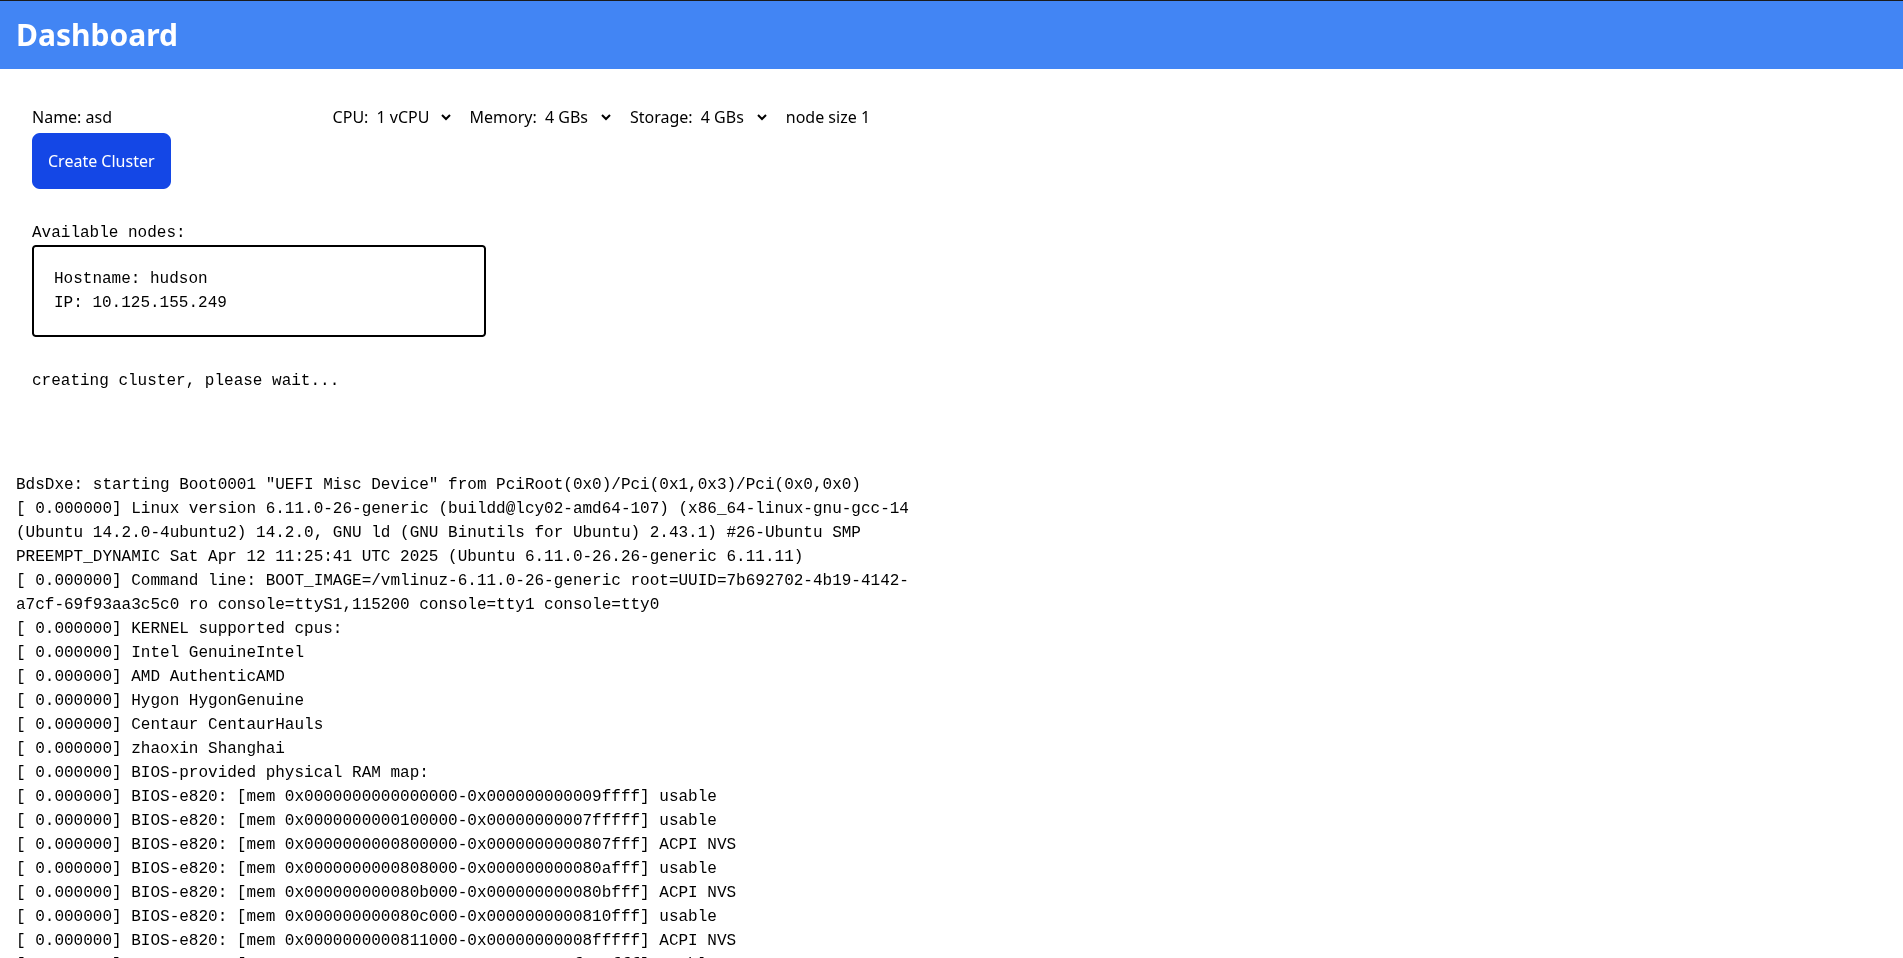
\includegraphics[scale=0.3]{gambar/website-create-process.png}}
  \caption{Proses Pembuatan Klaster}
  \label{fig:proses-pembuatan-klaster}
\end{figure}

\begin{figure}[H]
  \centering
  \fbox{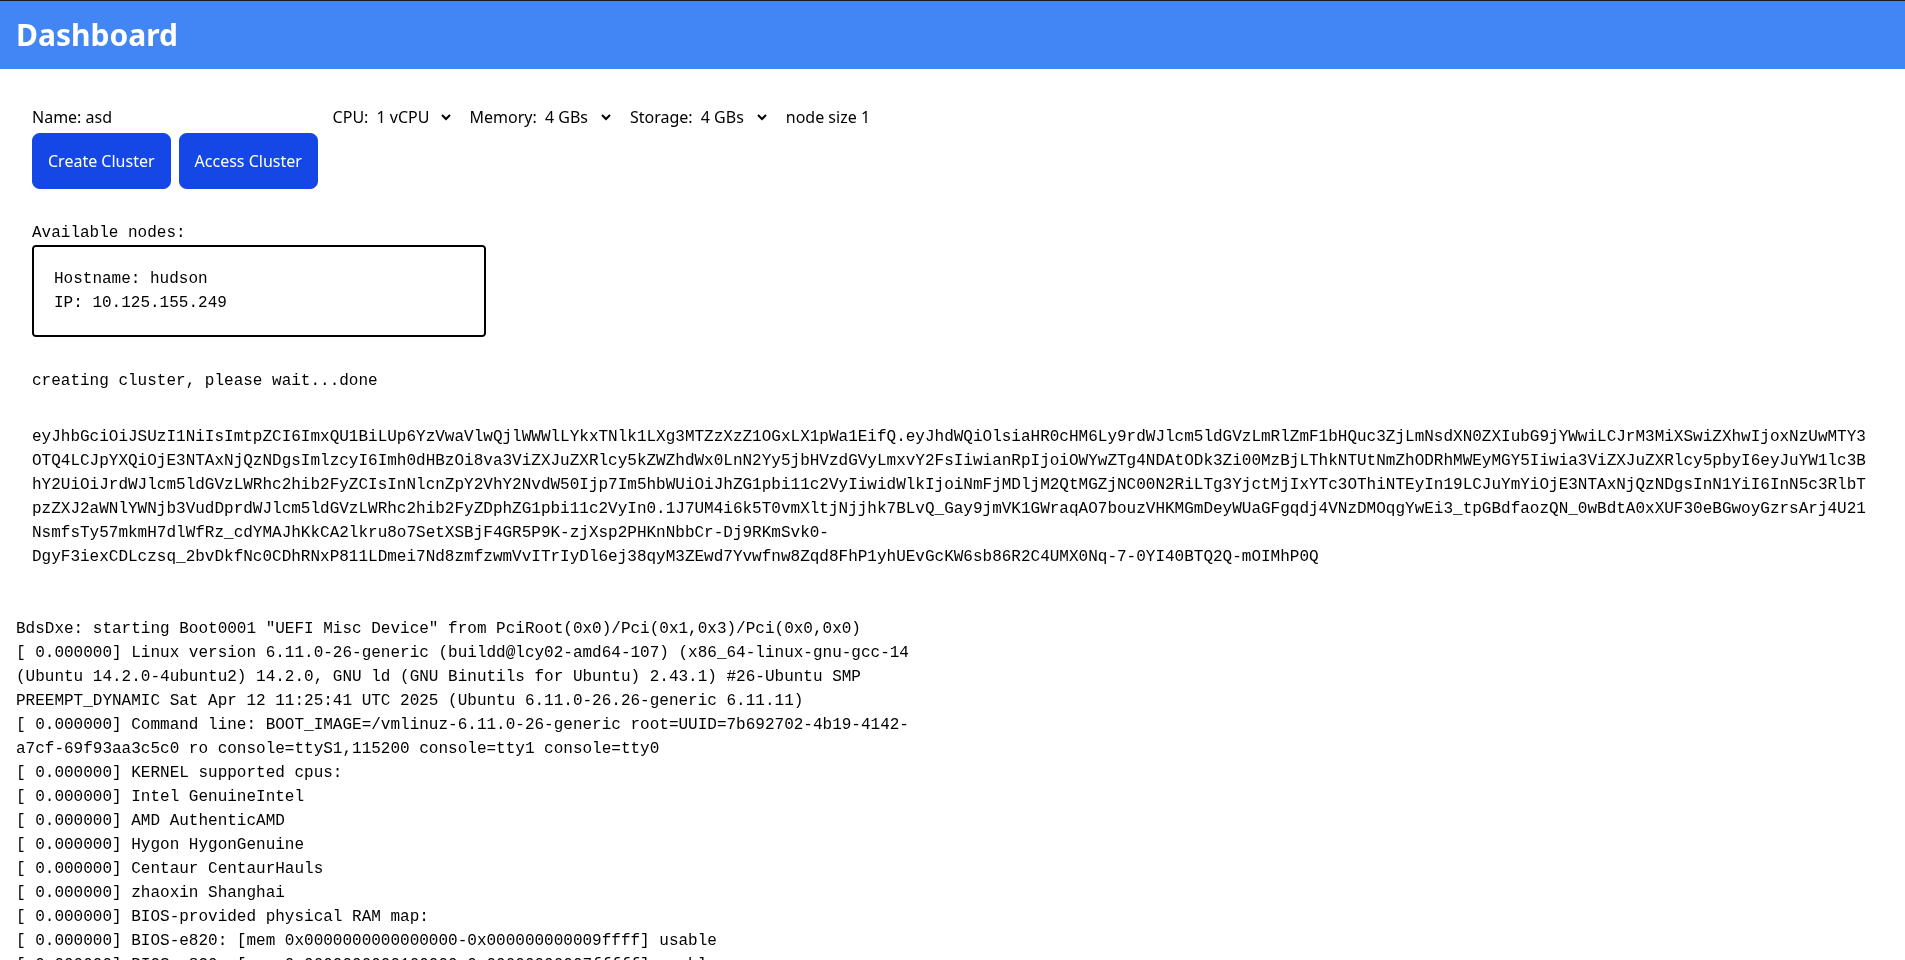
\includegraphics[scale=0.3]{gambar/website-create-process-done-local.png}}
  \caption{Proses Pembuatan Klaster Selesai}
  \label{fig:proses-pembuatan-klaster-selesai}
\end{figure}

\begin{figure}[H]
  \centering
  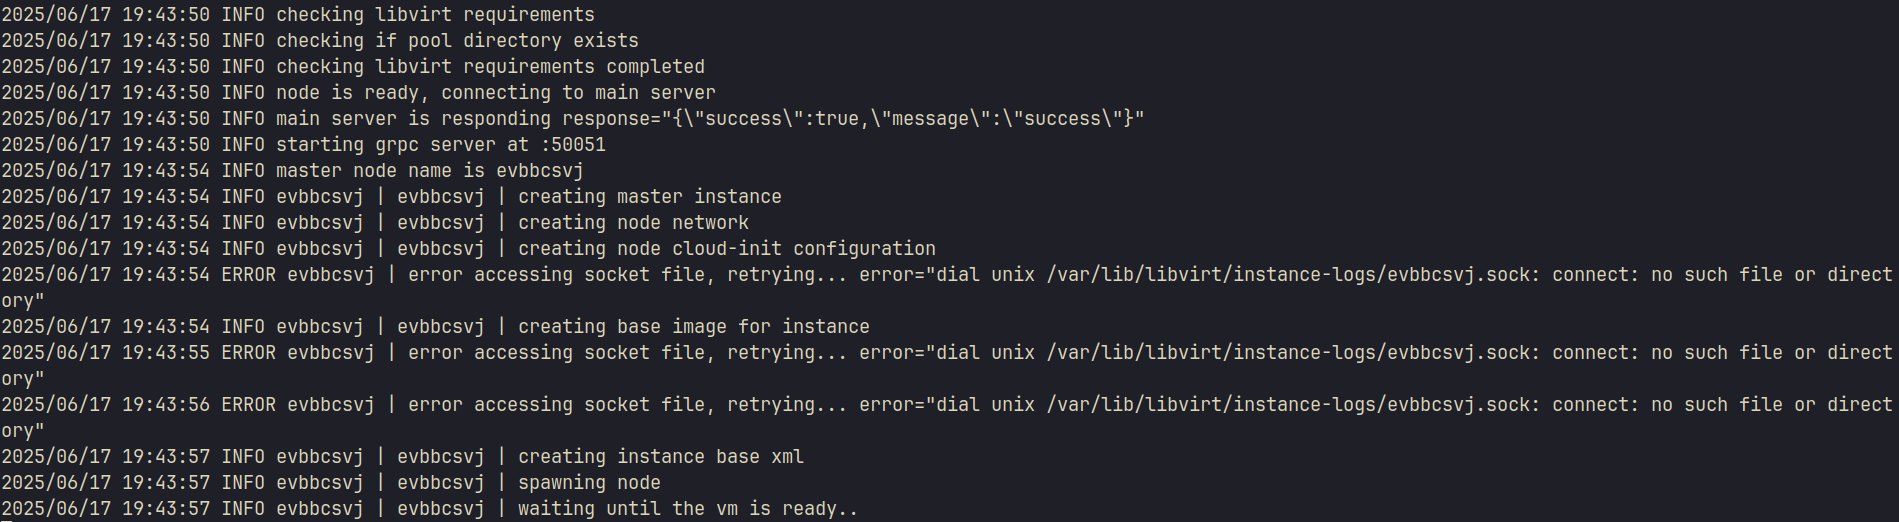
\includegraphics[scale=0.3]{gambar/worker-create-cluster-process-local.png}
  \caption{\emph{Log} pada Komputer \emph{Worker}}
  \label{fig:worker-create-cluster-process-local}
\end{figure}

\begin{figure}[H]
  \centering
  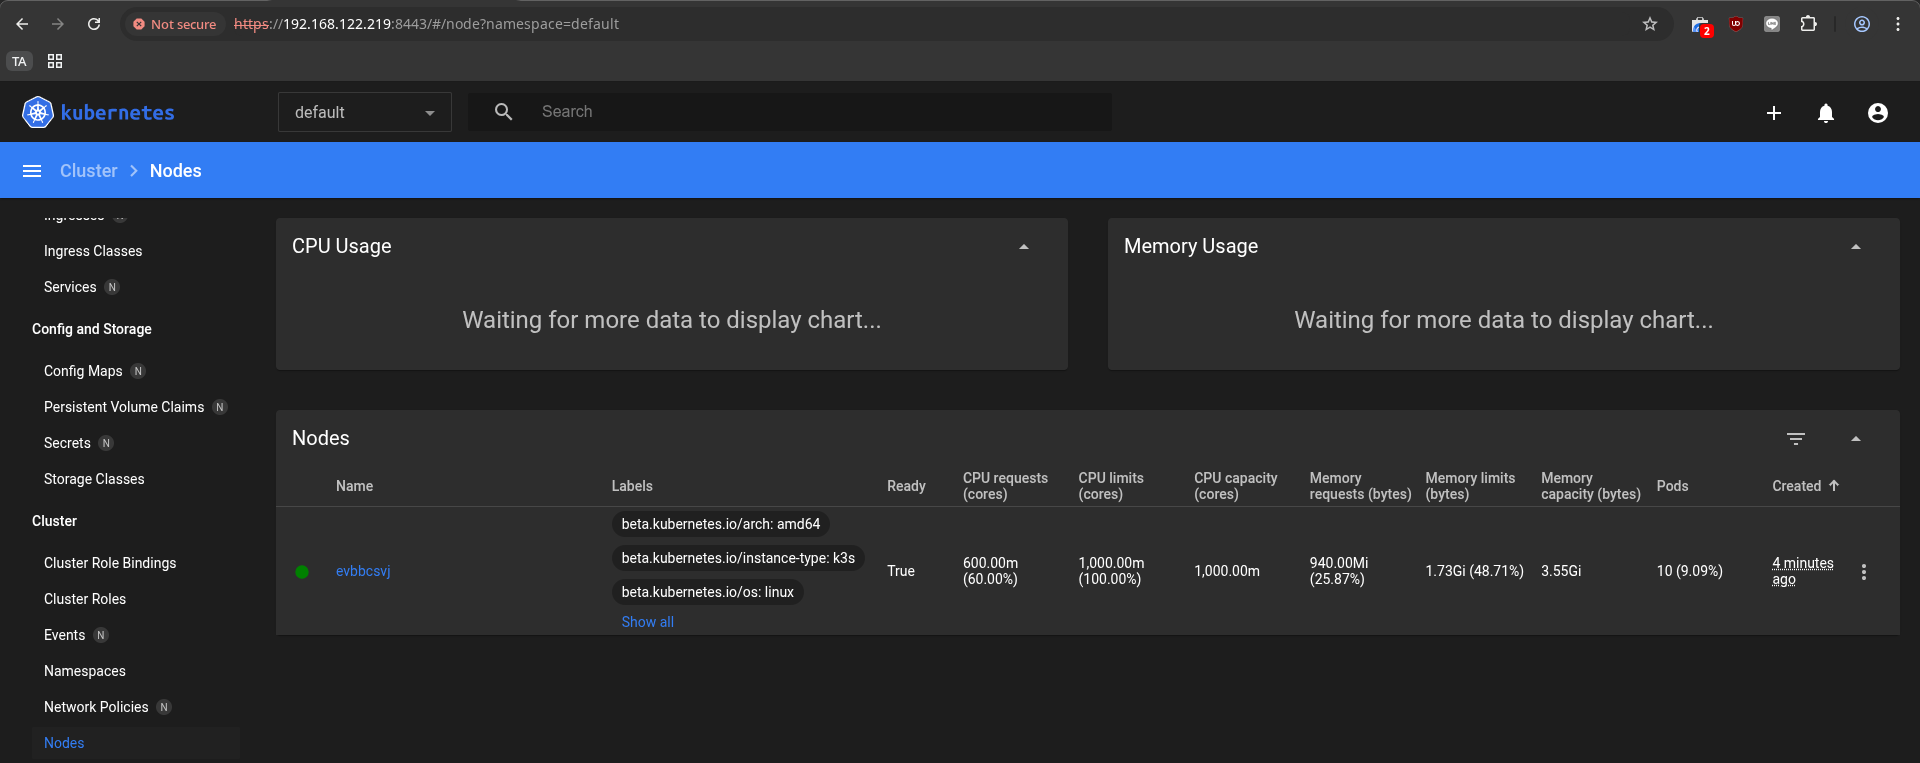
\includegraphics[scale=0.3]{gambar/kubernetes-dashboard-access-local-with-nodes.png}
  \caption{Daftar \emph{Nodes} pada Klaster dengan Satu \emph{Virtual Machine}}
  \label{fig:daftar-nodes-pada-dashboard-kubernetes}
\end{figure}

Berdasarkan gambar-gambar di atas, sistem \emph{provisioning} dapat membuat
\emph{virtual machine} yang secara otomatis tergabung dalam sebuah klaster Kubernetes.
Selain itu, \emph{control plane} juga menyediakan \emph{dashboard} Kubernetes yang dapat
digunakan oleh pengguna untuk berinteraksi dengan klaster Kubernetes tersebut.

\subsection{Pengujian Pembuatan \emph{Virtual Cluster} Lingkungan \emph{Production}}
\label{subsec:pengujian-pembuatan-vc-prod}

Pada lingkungan \emph{production}, \emph{virtual machine} yang tergabung dalam
satu klaster tidak selalu berada dalam satu komputer fisik \emph{worker} yang sama.
Pengujian dilakukan dengan cara membuat klaster berisi dua atau lebih \emph{virtual machine}
yang terdiri dari satu \emph{control plane} dan sisanya sebagai \emph{worker node}.
Semua \emph{Virtual machine} tersebut tidak selalu berada di komputer \emph{worker}
yang sama.

\subsubsection{\emph{Virtual Machine} di }

\subsubsection{\emph{Virtual Machine} di }

\subsection{\emph{Error Handling}}
\label{subsec:error-handling}

Proses \emph{provisioning virtual machine} untuk pembuatan
klaster Kubernetes tidak selalu berjalan baik. Terdapat banyak
faktor yang dapat membuat proses \emph{provisioning} gagal. Untuk
mengatasi hal tersebut, proses \emph{provisioning} pada implementasi
tugas akhir ini memiliki sifat atomik, yaitu jika terjadi \emph{error}
saat membuat \emph{virtual machine} dan \emph{virtual machine} sudah terbuat,
\emph{virtual machine} tersebut akan dihapus.

\lstinputlisting[
  language=go,
  style=codestyle,
  caption={Kode Sumber Penghapusan \emph{Virtual Machine}},
  label={lst:vm-delete-function}
]{program/delete-vm.go}

\lstinputlisting[
  language=go,
  style=codestyle,
  emphstyle=\color{black}\bfseries\underbar,
  emph={deleteInstance},
  caption={Contoh Penggunaan \emph{Error Handling}},
  label={lst:error-handling-example}
]{program/error-handling.go}

Pada kode sumber \ref{lst:vm-delete-function}, fungsi \lstinline{deleteInstance}
akan mematikan \emph{virtual machine} dan menghapus \emph{file} yang berkaitan
dengan \emph{virtual machine} tersebut seperti \emph{cloud image} yang dipakai.
Bentuk implementasi dari \emph{error handling} tersebut dapat dilihat pada kode
sumber \ref{lst:error-handling-example}. Pada kode sumber tersebut, jika terjadi
\emph{error} pada saat membuat \emph{virtual machine}, maka \emph{virtual machine}
tersebut akan dihapus beserta semua \emph{file} yang berkaitan.

% Contoh pembuatan tabel
% \begin{longtable}{|c|c|c|}
%   \caption{Hasil Pengukuran Energi dan Kecepatan}
%   \label{tb:EnergiKecepatan}                                   \\
%   \hline
%   \rowcolor[HTML]{C0C0C0}
%   \textbf{Energi} & \textbf{Jarak Tempuh} & \textbf{Kecepatan} \\
%   \hline
%   10 J            & 1000 M                & 200 M/s            \\
%   20 J            & 2000 M                & 400 M/s            \\
%   30 J            & 4000 M                & 800 M/s            \\
%   40 J            & 8000 M                & 1600 M/s           \\
%   \hline
% \end{longtable}

\cleardoublepage

% Bab 5 penutup
\chapter{KESIMPULAN DAN SARAN}
\label{chap:penutup}

Pada bab ini akan dipaparkan kesimpulan dari hasil implementasi
yang sudah dilakukan. Selain itu, saran mengenai hal yang dapat
dilakukan untuk mengembangkan implementasi ini juga akan dipaparkan.

\section{Kesimpulan}
\label{sec:kesimpulan}

Berdasarkan hasil implementasi yang dilakukan, berikut adalah
kesimpulan yang dapat diambil berdasarkan permasalahan yang diangkat
pada tugas akhir ini:

\begin{enumerate}[nolistsep]

  \item Pembuatan sistem \emph{provisioning} untuk menerapkan \emph{multi-tenancy}
    dalam klaster Kubernetes dapat dilakukan dengan cara mengaplikasikan \emph{tools}
    untuk membuat \emph{virtual machine} seperti Libvirt, Cloud-init, dan \emph{cloud images}.

  \item Penerapan \emph{multi-tenancy} pada implementasi ini adalah
    komputer fisik yang digunakan sebagai tempat \emph{provisioning} dapat
    membuat lebih dari satu \emph{virtual machine} yang tergabung dalam
    klaster yang berbeda. Implementasi tersebut menyebabkan komputer
    fisik tersebut melayani lebih dari satu \emph{user} sehingga
    komputer fisik tersebut memenuhi kriteria \emph{multi-tenancy}.

  \item Pembuatan \emph{virtual machine} yang secara otomatis tergabung
    dalam sebuah klaster Kubernetes dapat dicapai melalui beberapa \emph{tools}
    seperti K3s, Libvirt dan Cloud-init. K3s digunakan sebagai distribusi
    Kubernetes yang berukuran lebih kecil untuk membuat klaster Kubernetes,
    Libvirt digunakan untuk berinteraksi dengan hypervisor agar dapat membuat 
    \emph{virtual machine} dan Cloud-init digunakan untuk mengotomatisasi proses
    pembuatan dan penggabungan klaster Kubernetes.

\end{enumerate}

\section{Saran}
\label{chap:saran}

Untuk pengembangan lebih lanjut pada sistem \emph{provisioning}
untuk membuat klaster Kubernetes adalah sebagai berikut:

\begin{enumerate}[nolistsep]

  \item Meningkatkan kualitas dari antarmuka pengguna dan pengalaman
    pengguna pada situs web \emph{dashboard} sebagai antarmuka
    yang digunakan oleh \emph{user} untuk membuat klaster.

  \item Meningkatkan keamanan dengan cara mengisolasi \emph{virtual machine}
    agar tidak dapat diakses oleh \emph{virtual machine} lain yang tidak
    dalam satu klaster.

\end{enumerate}

\cleardoublepage

\chapter*{DAFTAR PUSTAKA}
\addcontentsline{toc}{chapter}{DAFTAR PUSTAKA}
\renewcommand\refname{}
\vspace{2ex}
\renewcommand{\bibname}{}
\begingroup
\def\chapter*#1{}
\printbibliography
\endgroup
\cleardoublepage

% Biografi penulis
\begin{center}
  \Large
  \textbf{BIOGRAFI PENULIS}
\end{center}

\addcontentsline{toc}{chapter}{BIOGRAFI PENULIS}

\vspace{2ex}

\begin{wrapfigure}{L}{0.3\textwidth}
  \centering
  \vspace{-3ex}
  % Ubah file gambar berikut dengan file foto dari mahasiswa
  
\includegraphics[width=0.3\textwidth]{gambar/elon.jpg}
  \vspace{-4ex}
\end{wrapfigure}

% Ubah kalimat berikut dengan biografi dari mahasiswa
\name{}, lahir pada 24 Agustus 2002

\cleardoublepage

\end{document}
